\documentclass[11pt,a4paper]{article}
\newcommand{\doctype}{Fiche étudiants}
% Style des documents du TP plaintes : celui des TP audio (style_bleu.tex), palette chocolat vers rouge. Les noms des couleurs (darkblue, skyblue...) sont gardés pour que les macros restent identiques.
% Repris de docs/style_bleu.tex ; seule la palette change.
% Chargé par input{style_chocolat} dans fiche_etudiants_plaintes.tex.
\usepackage[T1]{fontenc}
\usepackage[utf8]{inputenc}
\usepackage[french]{babel}
\frenchsetup{StandardItemLabels=true}
\usepackage{lmodern}
\usepackage{geometry}
\usepackage[table]{xcolor}
\usepackage{titlesec}
\usepackage{enumitem}
\usepackage{booktabs,tabularx,array}
\usepackage{fancyhdr}
\usepackage{tikz}
\usetikzlibrary{positioning,arrows.meta,fit,calc,decorations.pathreplacing}
\usepackage[most]{tcolorbox}
\usepackage{amsmath,amssymb}
\usepackage{graphicx}
\usepackage{multicol}
\usepackage{float}
\usepackage{pdflscape}
\usepackage{listings}
\usepackage{fontawesome5}
\usepackage{xurl}
\usepackage{hyperref}
\usepackage{microtype}

\geometry{margin=2.2cm, top=2.8cm, bottom=2.5cm}
\setlength{\headheight}{14pt}
\setlength{\emergencystretch}{3em}
\graphicspath{{figures/}{../figures/}}

% Palette chocolat vers rouge (noms des couleurs inchangés)
\definecolor{titlebg}{HTML}{5C3A2E}
\definecolor{sectioncolor}{HTML}{5C3A2E}
\definecolor{notebg}{HTML}{FBF1E8}
\definecolor{darkblue}{HTML}{3B2219}
\definecolor{accentblue}{HTML}{C0392B}
\definecolor{lightblue}{HTML}{E8765C}
\definecolor{skyblue}{HTML}{E4A857}
\definecolor{palblue}{HTML}{E9DCCF}
\definecolor{bgblue}{HTML}{FBF1E8}
\definecolor{formulabg}{HTML}{FDF8F3}
\definecolor{kpiblue}{HTML}{7B1E16}
\definecolor{codebg}{HTML}{F5F5F5}
\definecolor{codeframe}{HTML}{CCCCCC}
\definecolor{slate}{HTML}{8C776C}

\hypersetup{colorlinks=true, linkcolor=sectioncolor, urlcolor=sectioncolor, citecolor=sectioncolor}

\titleformat{\section}
  {\Large\bfseries\color{sectioncolor}}
  {\thesection.}{0.5em}{}
  [\vspace{-0.3em}{\color{accentblue}\titlerule[1.5pt]}]
\titleformat{\subsection}
  {\large\bfseries\color{sectioncolor}}
  {\thesubsection}{0.5em}{}

\pagestyle{fancy}
\fancyhf{}
\renewcommand{\headrulewidth}{1.5pt}
\renewcommand{\headrule}{\hbox to\headwidth{\color{accentblue}\leaders\hrule height \headrulewidth\hfill}}
\providecommand{\entete}{\textbf{École d'automne IA} \,|\, Hackathon voix du client}
\fancyhead[L]{\small\color{sectioncolor}\entete}
\fancyhead[R]{\small\color{sectioncolor}\doctype}
\fancyfoot[C]{\small\color{sectioncolor}\thepage}
\renewcommand{\footrulewidth}{0.5pt}
\renewcommand{\footrule}{\hbox to\headwidth{\color{skyblue}\leaders\hrule height \footrulewidth\hfill}}

\lstset{basicstyle=\ttfamily\small, backgroundcolor=\color{codebg}, frame=single,
  rulecolor=\color{codeframe}, columns=fullflexible, breaklines=true,
  keywordstyle=\color{sectioncolor}\bfseries, commentstyle=\color{slate}\itshape,
  stringstyle=\color{darkblue}, showstringspaces=false, language=Python,
  literate={é}{{\'e}}1 {è}{{\`e}}1 {à}{{\`a}}1 {ê}{{\^e}}1 {ç}{{\c c}}1 {ô}{{\^o}}1
    {î}{{\^i}}1 {ï}{{\"i}}1 {û}{{\^u}}1 {ù}{{\`u}}1 {â}{{\^a}}1 {ë}{{\"e}}1 {É}{{\'E}}1 {À}{{\`A}}1
    {«}{{\guillemotleft}}1 {»}{{\guillemotright}}1 {’}{{'}}1}

\newtcolorbox{notebox}[1][]{colback=notebg, colframe=sectioncolor, fonttitle=\bfseries,
  arc=3pt, boxrule=0.5pt, breakable, left=8pt, right=8pt, top=6pt, bottom=6pt, #1}
\newtcolorbox{conceptbox}[1][]{colback=white, colframe=sectioncolor!70!black, fonttitle=\bfseries,
  arc=3pt, boxrule=0.8pt, breakable, left=8pt, right=8pt, top=6pt, bottom=6pt, #1}
\newtcolorbox{kpibox}[1][]{colback=notebg, colframe=sectioncolor, coltitle=white,
  colbacktitle=titlebg, fonttitle=\bfseries, arc=3pt, boxrule=0.8pt, breakable,
  left=8pt, right=8pt, top=6pt, bottom=6pt, #1}
\newtcolorbox{formulabox}{colback=formulabg, colframe=skyblue, arc=2pt, boxrule=0.8pt,
  left=10pt, right=10pt, top=6pt, bottom=6pt}
\newtcolorbox{stepbox}[1][]{colback=white, colframe=accentblue, coltitle=white,
  colbacktitle=titlebg, fonttitle=\bfseries, arc=3pt, boxrule=0.8pt, breakable,
  left=8pt, right=8pt, top=6pt, bottom=6pt, #1}
\newtcolorbox{questionbox}{colback=notebg, colframe=darkblue, arc=3pt, boxrule=0.8pt,
  left=10pt, right=10pt, top=8pt, bottom=8pt}

% Explication « pour un enfant » : une image de la vie de tous les jours, avant le vrai mot
\newtcolorbox{enfant}[1][]{enhanced, colback=white, colframe=lightblue, boxrule=1.2pt, arc=6pt,
  left=40pt, right=10pt, top=6pt, bottom=6pt, breakable,
  overlay={\node[circle, fill=lightblue, text=white, minimum size=24pt, font=\large]
    at ([xshift=20pt]frame.west) {\faChild};}, #1}
% Le piège à éviter
\newtcolorbox{piege}[1][]{enhanced, colback=white, colframe=darkblue, boxrule=1.2pt, arc=6pt,
  left=40pt, right=10pt, top=6pt, bottom=6pt, breakable,
  overlay={\node[circle, fill=darkblue, text=white, minimum size=24pt, font=\large]
    at ([xshift=20pt]frame.west) {\faExclamationTriangle};}, #1}
% Un chiffre clé dans une pastille : \cle{1 446}{appels}
\newcommand{\cle}[2]{\tikz[baseline=(n.base)]\node[fill=notebg, draw=sectioncolor, rounded corners=4pt,
  inner sep=5pt, align=center, text width=2.35cm] (n) {{\Large\bfseries\color{darkblue}#1}\\[-1pt]{\footnotesize\color{slate}#2}};}
% Page « vue d'ensemble » : le pipeline complet en 3D (Three.js), placée après la page de titre
\newcommand{\vuedensemble}{%
\begin{landscape}
\section*{Vue d'ensemble : les modèles et la méthode}
\addcontentsline{toc}{section}{Vue d'ensemble : les modèles et la méthode}
\begin{center}
\includegraphics[width=\linewidth, height=12.2cm, keepaspectratio]{3d_ensemble.png}
\end{center}
\begin{tcbraster}[raster columns=3, raster equal height, raster column skip=6pt]
\begin{kpibox}[title={\faIcon{file-audio}\ 1. Préparer}, unbreakable]
\small Lire et convertir le son, savoir qui parle, découper les tours, transcrire, puis masquer noms et
numéros \textbf{avant tout modèle}.
\end{kpibox}
\begin{kpibox}[title={\faProjectDiagram\ 2. Des branches indépendantes}, unbreakable]
\small \textbf{A} les mots (TF-IDF), \textbf{A bis} les modèles pré-entraînés, \textbf{B} la voix,
\textbf{C} le déroulement : chacune donne un score, une fusion tardive les combine.
\end{kpibox}
\begin{kpibox}[title={\faBalanceScale\ 3. Juger honnêtement}, unbreakable]
\small Une étiquette auditée, un découpage sans tricher (par client, par date), un repère à battre
(0,637), puis l'ablation.
\end{kpibox}
\end{tcbraster}
\end{landscape}}

% Bandeau d'ouverture d'une grande partie
\newcommand{\bandeaupartie}[2]{\clearpage
\begin{tcolorbox}[colback=titlebg, colframe=titlebg, coltext=white, arc=5pt, boxrule=0pt,
  left=15pt, right=15pt, top=12pt, bottom=12pt]
\begin{center}{\Large\bfseries #1}\\[6pt]{\normalsize #2}\end{center}
\end{tcolorbox}}

\setlist[itemize]{leftmargin=1.5em, label={\color{sectioncolor}\textbullet}}
\setlist[enumerate]{leftmargin=1.5em, label={\color{sectioncolor}\arabic*.}}

% Page de titre commune : #1 sur-titre, #2 titre, #3 sous-titre, #4 ligne bleue, #5 objectif
\newcommand{\pagedetitre}[5]{%
\thispagestyle{empty}
\begin{tikzpicture}[remember picture, overlay]
  \fill[titlebg] (current page.north west) rectangle ([yshift=-8cm]current page.north east);
  \fill[lightblue] ([yshift=-8cm]current page.north west) rectangle ([yshift=-8.3cm]current page.north east);
  \fill[titlebg] (current page.south west) rectangle ([yshift=1.5cm]current page.south east);
  \fill[lightblue] ([yshift=1.5cm]current page.south west) rectangle ([yshift=1.8cm]current page.south east);
\end{tikzpicture}
\vspace*{0.1cm}
\begin{center}
  {\color{skyblue}\large\textbf{#1}}\\[0.5cm]
  {\color{white}\Huge\textbf{#2}}\\[0.4cm]
  {\color{palblue}\LARGE #3}\\[0.3cm]
  {\color{skyblue}\large #4}
\end{center}
\vspace*{1.6cm}
\begin{center}\couverture\end{center}
\vspace*{0.8cm}
\begin{center}
  \begin{tikzpicture}
    \node[fill=notebg, rounded corners=6pt, inner sep=14pt, text width=13cm, align=center,
      draw=sectioncolor, line width=0.8pt] {{\color{darkblue}\large\textbf{Objectif :} #5}};
  \end{tikzpicture}
\end{center}
\vfill
\begin{center}{\color{white}\small Année 2026-2027}\end{center}
\newpage
\setcounter{page}{1}}

% Illustration de couverture : le pipeline 1 en trois branches
\newcommand{\couverture}{%
\begin{tikzpicture}[
  b/.style={draw=##1, fill=##1!12, rounded corners=4pt, minimum width=3cm, minimum height=1.1cm,
    align=center, font=\small},
  a/.style={-{Stealth[length=2.5mm]}, thick, color=slate}]
\node[b=slate] (in) {{\Large\faPhone}\\Appel};
\node[b=darkblue, right=0.9cm of in] (d) {{\Large\faUsers}\\Qui parle ?};
\node[b=sectioncolor, right=0.9cm of d, yshift=1.5cm] (A) {{\Large\faFont}\\A : les mots};
\node[b=accentblue, right=0.9cm of d] (B) {{\Large\faWaveSquare}\\B : la voix};
\node[b=lightblue, right=0.9cm of d, yshift=-1.5cm] (C) {{\Large\faStopwatch}\\C : le rythme};
\node[b=darkblue, right=0.9cm of B] (out) {{\Large\faSmile\ \faFrown}\\Satisfait ?};
\draw[a] (in) -- (d); \foreach \x in {A,B,C} {\draw[a] (d) -- (\x); \draw[a] (\x) -- (out);}
\end{tikzpicture}}

\setlength{\parindent}{0pt}
\usetikzlibrary{shapes.misc}
\setlength{\headheight}{23pt}
% Fiche des étudiants du TP plaintes : visuelle, sans les réponses des réflexions (elles sont dans le guide
% de l'encadrante). Les « Tu dois voir » donnent un critère à vérifier, sans chiffre propre à une base.

\definecolor{cacao}{HTML}{A9705A}
\definecolor{bordeaux}{HTML}{7B1E16}
\definecolor{ambre}{HTML}{E4A857}

\newtcolorbox{card}[2]{colback=white, colframe=#1, coltitle=white, colbacktitle=#1,
  fonttitle=\bfseries\large, title={#2}, arc=3pt, boxrule=1pt, equal height group=cards,
  before upper=\raggedright}
\newtcolorbox{bloc}[2][sectioncolor]{colback=white, colframe=#1, coltitle=white,
  colbacktitle=#1, fonttitle=\bfseries, title={#2}, arc=3pt, boxrule=0.8pt,
  left=8pt, right=8pt, top=6pt, bottom=6pt}
\newtcolorbox{lire}[1][]{enhanced, colback=notebg, colframe=accentblue, boxrule=0.8pt, arc=4pt,
  left=40pt, right=10pt, top=6pt, bottom=6pt, breakable,
  overlay={\node[circle, fill=accentblue, text=white, minimum size=24pt, font=\large]
    at ([xshift=20pt]frame.west) {\faEye};}, #1}

% logo d'une organisation (figures/logos/)
\newcommand{\logo}[1]{\raisebox{-0.3\height}{\includegraphics[height=0.42cm]{logos/#1}}\,}
\newcommand{\chiffre}[1]{{\Large\bfseries\color{darkblue} #1}}
\newcommand{\doisvoir}[1]{\par\smallskip{\color{accentblue}\faCheckCircle\ \textbf{Tu dois voir :}} #1}
\newcommand{\image}[1]{\par\smallskip{\color{lightblue}\faChild}\ \textit{#1}}
\newcommand{\reflexion}[2]{\begin{questionbox}\textbf{\faQuestionCircle\ Réflexion #1.} #2\end{questionbox}}
% une image et sa légende, jamais séparées par un saut de page
\newcommand{\illus}[3][\linewidth]{\begin{center}\begin{minipage}{\linewidth}\centering
  \includegraphics[width=#1]{#2}\\[2pt]{\small\color{slate}\textit{#3}}\end{minipage}\end{center}}

% Couverture : la chaîne du TP plaintes
\renewcommand{\couverture}{%
\begin{tikzpicture}[
  b/.style={draw=##1, fill=##1!12, rounded corners=4pt, minimum width=2.45cm, minimum height=1.25cm,
    align=center, font=\small},
  a/.style={-{Stealth[length=2.5mm]}, thick, color=slate}]
\node[b=slate] (p) {{\Large\faEnvelopeOpenText}\\Plaintes};
\node[b=darkblue, right=0.45cm of p] (v) {{\Large\faProjectDiagram}\\Vecteurs};
\node[b=sectioncolor, right=0.45cm of v] (g) {{\Large\faObjectGroup}\\Problèmes};
\node[b=accentblue, right=0.45cm of g] (i) {{\Large\faExclamationTriangle}\\Incidents};
\node[b=lightblue, right=0.45cm of i] (t) {{\Large\faChartPie}\\Tableau de bord};
\draw[a] (p) -- (v); \draw[a] (v) -- (g); \draw[a] (g) -- (i); \draw[a] (i) -- (t);
\end{tikzpicture}}

\begin{document}

\pagedetitre{École d'automne IA, Alsace Tech}{Hackathon voix du client}
  {TP plaintes : regrouper pour repérer les incidents}{Fiche étudiants : la chaîne principale, puis la chaîne de comparaison}
  {transformer des plaintes écrites en plusieurs langues en problèmes nommés, puis repérer ceux qui
  explosent sur une marque et une période, sans jamais lire ni sortir un texte confidentiel.}

% Copyright (c) 2026 Selina Cheggour. Tous droits réservés. Voir le fichier LICENSE.
% Contexte, vue d'ensemble de la chaîne, mise en route sur Kaggle, règles de confidentialité.

\section{Le problème en une page}

Une entreprise agroalimentaire reçoit chaque mois des centaines de plaintes de consommateurs, dans
plusieurs pays et plusieurs langues. Chaque plainte est un court texte libre, le \textbf{verbatim},
accompagné d'un numéro de cas, de la marque (numérotée), du segment d'activité et de la période.
\textbf{Personne n'a classé ces textes.}

\begin{tcolorbox}[colback=notebg,colframe=sectioncolor,arc=3pt,halign=center,boxrule=1.5pt]
{\Large\faSearch\quad\bfseries Quand plusieurs consommateurs décrivent le même problème,}\\[2pt]
{\Large\bfseries peut-on les \textcolor{accentblue}{regrouper} et voir si ce problème se
\textcolor{accentblue}{concentre} sur une marque et une période ?}
\end{tcolorbox}

\begin{enfant}
\textbf{Comme le courrier d'une mairie.} Si dix habitants écrivent la même semaine que l'eau du robinet
a un goût bizarre, c'est sans doute une canalisation, pas dix coïncidences. Mais si la moitié de la
ville se plaint du froid en janvier, ce n'est pas une panne : c'est l'hiver. Et si mille lettres
identiques arrivent le même jour, c'est une pétition. Le TP apprend à faire la différence.
\end{enfant}

\subsection{Trois phénomènes qui se ressemblent, et qu'il faut séparer}

\begin{center}
\begin{tikzpicture}[x=0.32cm, y=0.13cm]
% trois mini-histogrammes : rouge = la marque concernée, beige = les autres marques
\foreach \nom/\dx/\titre/\coul in {inc/0/Incident/accentblue, sai/17/Saison/ambre, cam/34/Campagne/cacao} {
  \node[font=\bfseries, color=\coul] at (\dx+6.5,30) {\titre};
  \draw[slate!60] (\dx-0.5,0) -- (\dx+13.5,0);
}
% incident : une seule marque explose sur une période
\foreach \x/\a/\m in {0/3/0,1/2/1,2/4/0,3/3/1,4/2/0,5/3/0,6/3/16,7/4/2,8/2/0,9/3/1,10/2/0,11/3/0,12/2/0,13/3/1} {
  \fill[palblue] (\x-0.4,0) rectangle (\x+0.4,\a); \fill[accentblue] (\x-0.4,\a) rectangle (\x+0.4,\a+\m);}
% saison : toutes les marques montent ensemble
\foreach \x/\a/\m in {0/3/1,1/3/0,2/4/1,3/5/1,4/9/3,5/14/3,6/16/4,7/13/3,8/7/2,9/4/1,10/3/0,11/3/1,12/2/0,13/3/0} {
  \fill[palblue] (17+\x-0.4,0) rectangle (17+\x+0.4,\a); \fill[accentblue] (17+\x-0.4,\a) rectangle (17+\x+0.4,\a+\m);}
% campagne : un gros paquet de messages presque identiques
\foreach \x/\a/\m in {0/1/0,1/1/0,2/2/0,3/1/0,4/1/0,5/12/6,6/14/8,7/9/4,8/1/0,9/2/0,10/1/0,11/1/0,12/1/0,13/2/0} {
  \fill[palblue] (34+\x-0.4,0) rectangle (34+\x+0.4,\a); \fill[accentblue] (34+\x-0.4,\a) rectangle (34+\x+0.4,\a+\m);}
\node[font=\footnotesize, text width=4.9cm, align=center] at (6.5,-6) {une \textbf{seule marque} explose sur une ou deux périodes : un lot, une usine, une recette};
\node[font=\footnotesize, text width=4.9cm, align=center] at (23.5,-6) {\textbf{toutes les marques} montent ensemble : le chocolat fond l'été};
\node[font=\footnotesize, text width=4.9cm, align=center] at (40.5,-6) {des centaines de messages \textbf{presque identiques} : une mobilisation, pas un défaut};
\fill[accentblue] (12,-13) rectangle (12.8,-11.5); \node[right, font=\footnotesize] at (12.9,-12.2) {la marque signalée};
\fill[palblue] (24,-13) rectangle (24.8,-11.5); \node[right, font=\footnotesize] at (24.9,-12.2) {les autres marques};
\end{tikzpicture}
\end{center}
{\small\color{slate}\textit{Schéma inventé : une barre par période, pour un même problème.}}

\begin{tcbraster}[raster columns=3, raster equal height, raster column skip=6pt, raster every box/.style={unbreakable}]
\begin{kpibox}[title={\faExclamationTriangle\ Incident candidat}, unbreakable]
\small un problème en \textbf{excès} sur une case (marque, période), et cette marque porte au moins la
moitié du pic. \textbf{C'est ce qu'on cherche.}
\end{kpibox}
\begin{kpibox}[title={\faSun\ Pic partagé}, unbreakable]
\small un problème en excès sur une période, mais réparti entre les marques : une saison, un phénomène
général.
\end{kpibox}
\begin{kpibox}[title={\faBullhorn\ Campagne}, unbreakable]
\small un groupe dont la plupart des messages ont une jumelle \textbf{presque identique}.
\end{kpibox}
\end{tcbraster}

\begin{piege}
\textbf{Il n'y a pas d'étiquette.} On ne prédit rien : on \textbf{regroupe}. C'est de l'apprentissage
non supervisé, et toute la difficulté est de montrer que les groupes trouvés veulent dire quelque chose.
Le notebook travaille sur la \textbf{base réelle}. Les figures de cette fiche viennent d'une
\textbf{base fictive} de même forme, pour montrer à quoi ressemblent les résultats sans montrer de données
confidentielles.
\end{piege}

%%%%%%%%%%%%%%%%%%%%%%%%%%%%%%%%%%%%%%%%%%%%%%%%%%%%%%%%%%%%%%%%%%%%%%%%%%%%%%%%%%%%%%%%%%%%%%%%%%%%%%%%%
\newpage
\section{Deux grandes parties, dans cet ordre}

Le travail se fait en deux temps. D'abord la \textbf{chaîne principale} : un seul outil, de la lecture
du fichier jusqu'au tableau de bord. Ensuite seulement, une fois qu'elle marche, la \textbf{chaîne de
comparaison} : la même chaîne, rejouée avec huit outils.

\begin{center}
\begin{tikzpicture}[
  p/.style={draw=#1, fill=#1!10, rounded corners=6pt, minimum width=15.6cm, minimum height=1.3cm,
    text width=15.2cm, align=left, font=\small, inner sep=5pt},
  n/.style={circle, fill=#1, text=white, font=\bfseries, minimum size=0.9cm},
  gp/.style={fill=#1, text=white, rounded corners=4pt, font=\bfseries, minimum width=15.6cm, minimum height=0.8cm,
    text width=15.2cm, align=left, inner sep=5pt}]
\node[gp=sectioncolor] (g1) {\faRoute\quad Première grande partie : la chaîne principale \hfill{\normalfont\small un outil, Qwen3-Embedding-0.6B}};
\node[p=slate, below=0.25cm of g1] (p0) {\hspace{1.3cm}\parbox{13.7cm}{\textbf{Mise en route.} Carte graphique, internet, la base réelle attachée, outils et contrôles \texttt{verifier}.}};
\node[p=sectioncolor, below=0.25cm of p0] (p1) {\hspace{1.3cm}\parbox{13.7cm}{\textbf{Lire et contrôler.} Trouver l'en-tête tout seul, nettoyer les verbatims, compter, détecter la langue, chercher les données personnelles oubliées.}};
\node[p=darkblue, below=0.25cm of p1] (p2) {\hspace{1.3cm}\parbox{13.7cm}{\textbf{Transformer en vecteurs.} TF-IDF puis plongements multilingues ; retirer la \og signature \fg{} de chaque langue par centrage.}};
\node[p=accentblue, below=0.25cm of p2] (p3) {\hspace{1.3cm}\parbox{13.7cm}{\textbf{Regrouper.} HDBSCAN, fusion des groupes jumeaux d'une langue à l'autre, réglage automatique, mots et définitions de chaque problème, stabilité.}};
\node[p=lightblue, below=0.25cm of p3] (p4) {\hspace{1.3cm}\parbox{13.7cm}{\textbf{Repérer les incidents.} Plaintes observées contre attendues (loi de Poisson), correction des tests multiples, part de la marque dans le pic ; incident, saison ou campagne.}};
\node[p=cacao, below=0.25cm of p4] (p6) {\hspace{1.3cm}\parbox{13.7cm}{\textbf{Exporter.} \texttt{resultats.js} pour le tableau de bord, contrôlé : ni verbatim ni numéro de cas.}};
\node[draw=accentblue, fill=white, line width=1.2pt, rounded corners=12pt, below=0.35cm of p6, font=\small\bfseries,
  text=accentblue, inner sep=6pt] (porte) {\faCheckCircle\quad la chaîne principale est validée : ses vérifications lues, \texttt{resultats.js} écrit};
\node[gp=bordeaux, below=0.35cm of porte] (g2) {\faBalanceScale\quad Deuxième grande partie : la chaîne de comparaison \hfill{\normalfont\small huit outils}};
\node[p=bordeaux, below=0.25cm of g2] (p7) {\hspace{1.3cm}\parbox{13.7cm}{\textbf{Comparer les outils.} La même chaîne, du centrage aux alertes, avec huit représentations, du comptage de mots à un transformer de 4 milliards de paramètres : temps, mémoire, coût, qualité. Sortie : \texttt{comparaison.js}.}};
\node[p=slate, below=0.35cm of p7] (p8) {\hspace{1.3cm}\parbox{13.7cm}{\textbf{Pour finir : ce qui peut sortir de Kaggle.} Des chiffres seulement ; aucun texte ne s'affiche ni ne sort.}};
\foreach \k/\c in {0/slate,1/sectioncolor,2/darkblue,3/accentblue,4/lightblue,6/cacao,7/bordeaux,8/slate}
  \node[n=\c] at ($(p\k.west)+(0.75,0)$) {\k};
\draw[-{Stealth[length=3mm]}, very thick, color=accentblue] (p6) -- (porte);
\draw[-{Stealth[length=3mm]}, very thick, color=accentblue] (porte) -- (g2);
\end{tikzpicture}
\end{center}

\begin{enfant}
\textbf{Comme apprendre une recette avant d'acheter des casseroles.} On réussit d'abord le plat avec une
seule casserole (la chaîne principale). Ensuite seulement, on refait exactement la même recette avec huit
casseroles pour voir laquelle cuit le mieux, le plus vite et pour le moins cher (la chaîne de comparaison).
Comparer des casseroles sur une recette qu'on rate encore ne dirait rien.
\end{enfant}

%%%%%%%%%%%%%%%%%%%%%%%%%%%%%%%%%%%%%%%%%%%%%%%%%%%%%%%%%%%%%%%%%%%%%%%%%%%%%%%%%%%%%%%%%%%%%%%%%%%%%%%%%
\newpage
\section{Mise en route sur Kaggle}

\begin{bloc}[darkblue]{\faCalendarCheck\quad À faire AVANT la séance}
\begin{tikzpicture}[
  etape/.style={draw=darkblue,fill=white,rounded corners=4pt,minimum width=3.6cm,minimum height=1.5cm,
    align=center,font=\small,text width=3.4cm},
  arr/.style={-{Stealth[length=3mm]},very thick,color=darkblue}]
\node[etape] (a) {{\Large\faUserPlus}\\Créer un compte\\\textbf{kaggle.com}};
\node[etape,right=0.35cm of a] (b) {{\Large\faMobile*}\\\textbf{Vérifier ton téléphone}\\(sinon : ni GPU ni internet)};
\node[etape,right=0.35cm of b] (c) {{\Large\faFileImport}\\Importer le notebook\\du TP (\textbf{File, Import})};
\node[etape,right=0.35cm of c] (d) {{\Large\faDatabase}\\\textbf{Add Input} : le jeu\\de la base réelle};
\draw[arr] (a) -- (b); \draw[arr] (b) -- (c); \draw[arr] (c) -- (d);
\end{tikzpicture}
\end{bloc}

\begin{bloc}{\faPowerOff\quad Allumer le GPU et internet}
\begin{tikzpicture}[
  num/.style={circle,fill=sectioncolor,text=white,font=\bfseries\Large,minimum size=0.9cm},
  lab/.style={align=center,font=\small,text width=3.6cm},
  arr/.style={-{Stealth[length=3mm]},very thick,color=sectioncolor}]
\node[num] (n1) {1}; \node[num,right=3.0cm of n1] (n2) {2};
\node[num,right=3.0cm of n2] (n3) {3}; \node[num,right=3.0cm of n3] (n4) {4};
\node[lab,below=2pt of n1] {Panneau de droite :\\\textbf{Session options}};
\node[lab,below=2pt of n2] {\textbf{Accelerator}\\\faArrowRight\ \textbf{GPU T4}};
\node[lab,below=2pt of n3] {\textbf{Internet}\\\faToggleOn\ \textbf{On}};
\node[lab,below=2pt of n4] {Exécuter les cellules\\de la \textbf{partie 0}};
\draw[arr] (n1) -- (n2); \draw[arr] (n2) -- (n3); \draw[arr] (n3) -- (n4);
\end{tikzpicture}
\end{bloc}

\begin{tcbraster}[raster columns=2, raster equal height, raster column skip=8pt, raster every box/.style={unbreakable}]
\begin{enfant}[unbreakable]
\textbf{Internet sert à télécharger les modèles} (des fichiers de plusieurs centaines de mégaoctets
à quelques gigaoctets), jamais à envoyer les plaintes : tous les calculs se font dans le notebook.
\end{enfant}
\begin{enfant}[unbreakable]
\texttt{[À revoir]} = la marge d'une copie corrigée : une remarque et un \textbf{indice}, au lieu d'une
erreur qui arrête tout. \textbf{Lis l'indice} avant de passer à la suite.
\end{enfant}
\end{tcbraster}

\clearpage
\section{Les règles de confidentialité}

Le notebook tourne sur des plaintes réelles, couvertes par un accord de confidentialité que tu as signé.
Les règles ci-dessous s'appliquent donc à chaque exécution.

\begin{center}
\resizebox{\linewidth}{!}{%
\begin{tikzpicture}[
  z/.style={draw=#1, fill=#1!8, rounded corners=8pt, minimum height=3.5cm, text width=4.1cm, align=center, font=\small},
  f/.style={-{Stealth[length=3mm]}, very thick, color=#1}]
\node[z=darkblue] (k) {{\huge\faLock}\\[3pt]\textbf{Kaggle, en privé}\\[3pt]les verbatims, les numéros de cas, les vecteurs, les mots des problèmes\\[3pt]\textit{tout reste ici}};
\node[z=accentblue, right=1.7cm of k] (e) {{\huge\faShield*}\\[3pt]\textbf{L'export contrôlé}\\[3pt]\texttt{resultats.js}, \texttt{comparaison.js} : des chiffres seulement\\[3pt]\textit{refusé s'il contient un numéro de cas ou un verbatim}};
\node[z=lightblue, right=1.7cm of e] (t) {{\huge\faChartPie}\\[3pt]\textbf{Le tableau de bord}\\[3pt]sur ta machine, sans internet\\[3pt]\textit{les problèmes y sont numérotés}};
\draw[f=darkblue] (k) -- node[above, font=\footnotesize] {calcul} (e);
\draw[f=accentblue] (e) -- node[above, font=\footnotesize] {téléchargement} (t);
\end{tikzpicture}}
\end{center}

\begin{tikzpicture}[
  rule/.style={draw=#1,fill=#1!10,rounded corners=5pt,minimum height=1.75cm,
    text width=7.55cm,align=left,font=\normalsize,inner sep=8pt},
  ico/.style={font=\Huge,color=#1}]
\node[rule=sectioncolor] (r1) at (0,0) {\hspace{1.4cm}\parbox{5.95cm}{\textbf{Ne recopie aucun verbatim}\\
  ni dans un rapport, ni dans un message, ni dans une capture d'écran.}};
\node[ico=sectioncolor] at ($(r1.west)+(0.8,0)$) {\faCopy};
\node[rule=accentblue,right=0.3cm of r1] (r2) {\hspace{1.4cm}\parbox{5.95cm}{\textbf{Aucun service en ligne}\\
  pour lire ou traduire les plaintes : pas de chatbot, pas de traducteur web.}};
\node[ico=accentblue] at ($(r2.west)+(0.8,0)$) {\faCloud};
\node[rule=darkblue,below=0.3cm of r1] (r3) {\hspace{1.4cm}\parbox{5.95cm}{\textbf{Notebook privé.}\\
  Jamais \og Public \fg{}, jamais partagé hors de l'équipe.}};
\node[ico=darkblue] at ($(r3.west)+(0.8,0)$) {\faUserSecret};
\node[rule=lightblue,below=0.3cm of r2] (r4) {\hspace{1.4cm}\parbox{5.95cm}{\textbf{Ne télécharge que l'export}\\
  (\texttt{tableau\_de\_bord/*.js}), jamais les vecteurs \texttt{plongements\_*.npy} : on sait parfois
  retrouver une partie d'un texte à partir de son vecteur.}};
\node[ico=lightblue] at ($(r4.west)+(0.8,0)$) {\faDownload};
\end{tikzpicture}

% Copyright (c) 2026 Selina Cheggour. Tous droits réservés. Voir le fichier LICENSE.
% Parties 0 à 2 du notebook : mise en route, lire et contrôler le fichier, transformer en vecteurs.

\bandeaupartie{I. Parties 0 à 2 : lire, nettoyer, transformer en nombres}{Avant de regrouper quoi que ce soit, on vérifie ce qu'on a reçu.}

\section{Partie 0 : mise en route}

\begin{stepbox}[title={\faPlay\quad Trois cellules, rien à modifier}]
\begin{tabularx}{\linewidth}{>{\bfseries\color{sectioncolor}}c X}
0.1 & \faDatabase\ \texttt{NOM\_FICHIER} : le fichier de la base réelle, déjà écrit. \texttt{AFFICHER\_TEXTES} vaut \texttt{False} : aucun verbatim ne s'affiche. \\
0.2 & \faPuzzlePiece\ installe \texttt{py3langid}, le détecteur de langue, et \texttt{babel}, pour le nom des langues en clair. \\
0.3 & \faToolbox\ charge les outils : \texttt{verifier}, la palette des graphiques, \texttt{montrer} qui range chaque figure dans \texttt{figures/}. \\
\end{tabularx}
\doisvoir{\texttt{Base : RÉELLE (aucun verbatim ne sera affiché)} et le nom du fichier réel, puis \texttt{Outils prêts.}}
\end{stepbox}

\section{Partie 1 : lire le fichier sans le connaître à l'avance}

L'export de l'entreprise est un tableau Excel qui n'est pas \og propre \fg{}.

\begin{center}
\resizebox{\linewidth}{!}{%
\begin{tikzpicture}[x=1cm, y=0.58cm, font=\small]
\foreach \c/\x/\w in {A/0/2.2,B/2.2/6.4,C/8.6/1.9,D/10.5/2.2,E/12.7/1.6,F/14.3/1.2} {
  \node[font=\footnotesize\bfseries, color=slate] at (\x+\w/2, 0.6) {\c};
}
\foreach \r in {1,...,9} \node[font=\footnotesize\bfseries, color=slate] at (-0.4,-\r+0.5) {\r};
\fill[notebg] (0,-2) rectangle (15.5,0); \node[color=slate, font=\footnotesize\itshape] at (7.7,-1) {lignes 1 et 2 : vides};
\fill[sectioncolor!25] (0,-3) rectangle (15.5,-2);
\foreach \t/\x/\w in {Case Number/0/2.2,Verbatim/2.2/6.4,Brand/8.6/1.9,Business Segment/10.5/2.2,Year Period/12.7/1.6,Blank/14.3/1.2}
  \node[font=\footnotesize\bfseries, color=darkblue] at (\x+\w/2,-2.5) {\t};
\foreach \r/\num/\verb/\mq/\seg/\per in {3/10001234/{EXTERNALBonjour,j'ai acheté...}/Brand 003/Chocolate/26 P05,
  4/10001302/{EXTERNALHello,the bar *******...}/Brand 007/Chocolate/26 P05,
  5/10001377/{EXTERNALGuten Tag,die Packung...}/Brand 012/Food/26 P06} {
  \node[anchor=west, font=\scriptsize\ttfamily] at (0.05,-\r-0.5) {\num};
  \node[anchor=west, font=\scriptsize\ttfamily] at (2.25,-\r-0.5) {\verb};
  \node[anchor=west, font=\scriptsize] at (8.65,-\r-0.5) {\mq};
  \node[anchor=west, font=\scriptsize] at (10.55,-\r-0.5) {\seg};
  \node[anchor=west, font=\scriptsize] at (12.75,-\r-0.5) {\per};
  \node[font=\scriptsize] at (14.9,-\r-0.5) {$\blacksquare$};
}
\node[color=slate, font=\footnotesize\itshape] at (7.7,-6.5) {\ldots\ des centaines de lignes \ldots};
\fill[notebg] (0,-9) rectangle (15.5,-7); \node[color=slate, font=\footnotesize\itshape] at (7.7,-8) {lignes vides en fin de tableau};
\draw[slate!50] (0,-9) grid[xstep=15.5, ystep=1] (15.5,0);
\foreach \x in {2.2,8.6,10.5,12.7,14.3} \draw[slate!50] (\x,0) -- (\x,-9);
\draw[accentblue, very thick, rounded corners] (14.25,-9.1) rectangle (15.55,0.1);
\node[accentblue, font=\footnotesize\bfseries, anchor=north] at (14.9,-9.2) {à ignorer};
\draw[-{Stealth}, accentblue, thick] (-1.6,-2.5) node[left, font=\footnotesize\bfseries, text width=1.6cm, align=right] {l'en-tête est en ligne 3} -- (-0.7,-2.5);
\end{tikzpicture}}
\end{center}
{\small\color{slate}\textit{Schéma de la disposition du fichier ; les lignes montrées sont inventées.}}

\begin{stepbox}[title={1.1\quad Un lecteur qui trouve tout seul où commencent et finissent les données}]
\texttt{charger\_plaintes(chemin)} lit le fichier \textbf{sans en-tête et en texte}, cherche la première
ligne qui contient à la fois \texttt{Case Number} et \texttt{Verbatim}, garde les cinq colonnes utiles,
ignore \texttt{Blank} et les colonnes sans nom, retire les lignes vides, et rend un petit
\textbf{rapport} (feuille, ligne d'en-tête, lignes vides retirées, colonnes ignorées).
\doisvoir{l'en-tête trouvé tout seul (en \textbf{ligne 3} sur l'export), le nombre de plaintes lues, la colonne \texttt{Blank} ignorée, les cinq colonnes attendues et seulement elles.}
\image{un facteur qui cherche le nom sur l'enveloppe, au lieu de compter \og troisième enveloppe en partant du haut \fg.}
\end{stepbox}

\begin{piege}
\texttt{pd.read\_excel(chemin, skiprows=2, nrows=1301)} marche aujourd'hui, et \textbf{cassera en silence}
demain : une ligne de titre en plus ou un fichier plus long, et on lit de travers sans aucun message.
\end{piege}

\reflexion{1.1}{Si la prochaine livraison compte 40\,000 lignes, avec une ligne de titre en plus avant
l'en-tête, ou arrive en CSV avec un séparateur \texttt{;}, que faut-il changer dans
\texttt{charger\_plaintes} ? Et dans la version \texttt{skiprows=2, nrows=1301} ?}

\begin{stepbox}[title={1.2\quad Nettoyer les verbatims, dans le bon ordre}]
\begin{center}
\begin{tikzpicture}[
  t/.style={draw=#1, fill=#1!8, rounded corners=4pt, text width=13.8cm, align=left, font=\footnotesize\ttfamily, inner sep=5pt},
  e/.style={font=\footnotesize, color=slate, text width=13.8cm, align=center}]
\node[t=slate] (a) {EXTERNALBonjour,j'ai acheté une tablette ******* hier.Elle avait un goût de savon !Lien : https://exemple.org/fiche.produit};
\node[e, below=0.35cm of a] (s) {1. retirer \texttt{EXTERNAL} \quad 2. retirer le lien \quad 3. retirer les étoiles\\ 4. une espace après la ponctuation \quad 5. des espaces simples};
\node[t=accentblue, below=0.35cm of s] (b) {Bonjour, j'ai acheté une tablette hier. Elle avait un goût de savon ! Lien :};
\draw[-{Stealth[length=3mm]}, very thick, color=accentblue] (s.west) ++(-0.2,0.3) -- ++(0,-0.6);
\end{tikzpicture}
\end{center}
{\small\color{slate}\textit{Exemple inventé, dans la forme des verbatims de la base fictive.}}
\doisvoir{plus aucun texte ne commence par \texttt{EXTERNAL}, plus d'étoiles ni de liens, les phrases sont séparées, une adresse web n'est pas coupée en morceaux.}
\image{on enlève l'étiquette collée sur la lettre avant de la lire, et on sépare les mots écrits sans espace.}
\end{stepbox}

\reflexion{1.2}{Pourquoi retirer le lien \textbf{avant} de remettre des espaces après la ponctuation ?}

\begin{stepbox}[title={1.3\quad Contrôler ce qu'on a reçu}]
Doublons de \texttt{Case Number}, verbatims vides, longueur des textes en mots, comptes par marque, segment et période.
\doisvoir{aucun doublon, aucun verbatim vide ; la longueur médiane des plaintes, puis le nombre de marques, de segments et de périodes.}
\end{stepbox}

\illus[0.97\linewidth]{1_plaintes_par_periode.png}{Figure 1 du notebook (base fictive) : le nombre de plaintes par période.}

\begin{lire}
\textbf{Comment lire ce graphique.} Une barre par période (\og 26 P05 \fg{} : année 2026, cinquième période).
La ligne pointillée est la moyenne ; les barres rouges la dépassent de plus d'un quart. Ce graphique dit
\textbf{quand} il y a eu beaucoup de plaintes, jamais \textbf{pourquoi}.
\end{lire}

\reflexion{1.3}{Le graphique montre des bosses, l'été 2025 et au printemps 2026. Est-ce un incident ?}

\begin{stepbox}[title={1.4\quad Quelles langues ?}]
\texttt{py3langid.classify(texte)} rend le code de la langue et un score. La base n'a ni colonne pays ni
colonne langue : la langue est le seul indice de géographie.
\doisvoir{une langue pour chaque plainte, et \textbf{plusieurs langues} (les plaintes viennent d'Europe et du Moyen-Orient), de la plus fréquente à la plus rare, avec leur nom en clair. Quelques langues très rares sont souvent des erreurs du détecteur sur des textes courts.}
\image{la langue d'une lettre dit dans quelle boîte de tri la mettre, pas de quelle ville elle vient : l'allemand couvre plusieurs pays.}
\end{stepbox}

\begin{stepbox}[title={1.5\quad L'anonymisation a-t-elle laissé passer quelque chose ?}]
On \textbf{compte}, sans lire les textes, les verbatims d'origine qui contiennent encore une forme reconnaissable :
\begin{center}\small
\renewcommand{\arraystretch}{1.25}
\begin{tabular}{ll}
\toprule
\textbf{motif} & \textbf{expression régulière} \\
\midrule
adresse électronique & \verb|[\w.+-]+@[\w-]+\.[\w.]+| \\
numéro de téléphone & \verb|\+?\d[\d .-]{7,}\d| \\
suite d'au moins six chiffres & \verb|\b\d{6,}\b| \\
adresse web & \verb|https?://\S+| \\
\bottomrule
\end{tabular}
\end{center}
\doisvoir{ni courriel, ni téléphone, ni longue suite de chiffres ; \textbf{40 plaintes} contiennent un lien web ; toutes citent un produit masqué par des étoiles.}
\end{stepbox}

\reflexion{1.5}{Sur la base réelle, un compte non nul ne prouve pas une fuite, et un compte nul ne prouve
pas l'absence de fuite. Pourquoi ?}

%%%%%%%%%%%%%%%%%%%%%%%%%%%%%%%%%%%%%%%%%%%%%%%%%%%%%%%%%%%%%%%%%%%%%%%%%%%%%%%%%%%%%%%%%%%%%%%%%%%%%%%%
\clearpage
\section{Partie 2 : transformer chaque plainte en vecteur}

Pour regrouper des textes, il faut les transformer en nombres. Deux familles s'opposent.

\begin{center}
\resizebox{\linewidth}{!}{%
\begin{tikzpicture}[font=\small]
\begin{scope}
\node[font=\bfseries, color=sectioncolor] at (2.2,4.4) {TF-IDF : un axe par mot};
\draw[-{Stealth}, thick, slate] (0,0) -- (4.2,0) node[right] {\texttt{savon}};
\draw[-{Stealth}, thick, slate] (0,0) -- (0,3.8) node[above] {\texttt{Seife}};
\draw[-{Stealth}, thick, slate] (0,0) -- (-1.9,-1.6) node[below left] {\texttt{soap}};
\fill[accentblue] (3.2,0) circle (3pt) node[above, font=\footnotesize] {plainte FR};
\fill[ambre] (0,2.9) circle (3pt) node[right, font=\footnotesize] {plainte DE};
\fill[darkblue] (-1.4,-1.18) circle (3pt) node[right, font=\footnotesize] {plainte EN};
\node[text width=5.4cm, align=center, font=\footnotesize, color=slate] at (2.0,-2.7) {trois mots sans rapport : les trois plaintes sont à angle droit, aussi loin que possible};
\end{scope}
\begin{scope}[xshift=9.3cm]
\node[font=\bfseries, color=accentblue] at (1.8,4.4) {plongement : un espace de sens};
\fill[notebg] (1.8,1.7) ellipse (2.3 and 1.6);
\node[font=\footnotesize\itshape, color=slate] at (1.8,3.0) {\og goût de savon \fg};
\fill[accentblue] (1.4,1.6) circle (3pt) node[left, font=\footnotesize] {FR};
\fill[ambre] (2.1,1.9) circle (3pt) node[right, font=\footnotesize] {DE};
\fill[darkblue] (1.8,1.2) circle (3pt) node[below, font=\footnotesize] {EN};
\fill[slate] (4.4,-0.6) circle (3pt) node[right, font=\footnotesize] {\og emballage abîmé \fg};
\node[text width=5.4cm, align=center, font=\footnotesize, color=slate] at (1.9,-2.7) {un modèle entraîné sur plus de cent langues place les trois plaintes côte à côte};
\end{scope}
\end{tikzpicture}}
\end{center}

\begin{stepbox}[title={2.1\quad TF-IDF, et à quoi ressemblent les plus proches voisins}]
Chaque plainte $a$ devient un vecteur avec une coordonnée par terme $t$ :
\begin{formulabox}
\[
w_{t,a} = \bigl(1 + \ln \mathrm{tf}_{t,a}\bigr)\left(\ln\frac{1+n}{1+n_t} + 1\right)
\quad\text{si } \mathrm{tf}_{t,a} > 0, \qquad w_{t,a} = 0 \text{ sinon},
\]
où $\mathrm{tf}_{t,a}$ est le nombre de fois où $t$ apparaît dans la plainte $a$, $n$ le nombre de plaintes et
$n_t$ le nombre de plaintes qui contiennent $t$. Le vecteur est ensuite divisé par sa longueur. La
proximité de deux plaintes est le \textbf{cosinus} de leurs vecteurs $\mathbf{x}_a$, $\mathbf{x}_b$ :
$\cos(\mathbf{x}_a,\mathbf{x}_b) = \mathbf{x}_a^{\top}\mathbf{x}_b / (\lVert\mathbf{x}_a\rVert\,\lVert\mathbf{x}_b\rVert)$,
qui vaut 1 pour deux textes identiques et 0 pour deux textes sans mot commun.
\end{formulabox}
\illus[0.62\linewidth]{ill_tfidf.png}{Exemple inventé : un mot rare et répété pèse lourd, un mot partout (\og le \fg) presque rien.}
Ensuite, pour chaque plainte, on cherche sa plus proche voisine et on compte la part des plaintes dont la
voisine est \textbf{dans la même langue}.
\doisvoir{\textbf{757 mots} dans le vocabulaire ; voisine dans la même langue : \textbf{100 \%}.}
\end{stepbox}

\begin{stepbox}[title={2.2\quad Plongements multilingues : un transformer qui lit la plainte}]
\begin{center}
\resizebox{\linewidth}{!}{%
\begin{tikzpicture}[
  bx/.style={draw=#1, fill=#1!10, rounded corners=4pt, align=center, font=\footnotesize, minimum height=1.3cm},
  fl/.style={-{Stealth[length=2.5mm]}, thick, color=slate}]
\node[bx=slate, text width=3.2cm] (t) {\og Elle avait un goût de savon ! \fg};
\node[bx=sectioncolor, right=0.5cm of t, text width=2.8cm] (j) {jetons\\\texttt{Elle|avait|un|}\\\texttt{goût|de|sav|on|!}};
\node[bx=darkblue, right=0.5cm of j, text width=2.6cm] (m) {{\Large\faLayerGroup}\\28 couches d'attention};
\node[bx=accentblue, right=0.5cm of m, text width=2.6cm] (v) {un vecteur de\\\textbf{1\,024 nombres}};
\draw[fl] (t) -- (j); \draw[fl] (j) -- (m); \draw[fl] (m) -- (v);
\end{tikzpicture}}
\end{center}
Le modèle \texttt{Qwen/Qwen3-Embedding-0.6B} (Apache 2.0, plus de cent langues) reçoit chaque plainte
précédée d'une consigne (\og identifie le problème décrit \fg) et rend un vecteur de longueur 1. Dans
chaque couche, chaque jeton \og regarde \fg{} tous les autres pour préciser son sens : c'est
l'\textbf{attention}. Si le modèle ne se charge pas, la cellule passe à \texttt{multilingual-e5-base}.
\doisvoir{un vecteur normé par plainte ; voisine dans la même langue : \textbf{100 \%}, comme le TF-IDF.}
\image{un interprète qui résume chaque lettre en une \og empreinte de sens \fg, quelle que soit sa langue.}
\end{stepbox}

\reflexion{2.2}{Le plongement multilingue rapproche-t-il vraiment des plaintes de langues différentes ?
Regarde le pourcentage.}

\begin{stepbox}[title={2.3\quad Retirer la signature de la langue : le centrage}]
\begin{formulabox}
\[
\tilde{\mathbf{e}}_i = \frac{\mathbf{e}_i - \boldsymbol{\mu}_{\ell(i)}}{\lVert \mathbf{e}_i - \boldsymbol{\mu}_{\ell(i)} \rVert},
\]
où $\mathbf{e}_i$ est le plongement de la plainte $i$, $\ell(i)$ sa langue, et $\boldsymbol{\mu}_\ell$ la moyenne
des plongements des plaintes de la langue $\ell$. Une langue de moins de 10 plaintes reçoit la moyenne de
toutes les plaintes.
\end{formulabox}
\illus[0.92\linewidth]{ill_centrage.png}{Exemple inventé : la couleur est la langue, la forme le sujet. À gauche, on voit d'abord les langues ; à droite, après centrage, les sujets.}
\image{trois personnes qui parlent fort, doucement et avec un accent : on retire à chacune sa façon de
parler, et il ne reste que ce qu'elle dit.}
\doisvoir{un vecteur centré et normé par plainte ; voisine dans la même langue : \textbf{98 \%}, un peu moins qu'avant.}
\end{stepbox}

\illus[0.98\linewidth]{2_carte_langues_avant_apres.png}{Figure 2 du notebook (base fictive) : les plaintes en deux dimensions (t-SNE), avant et après centrage.}

\begin{lire}
\textbf{Comment lire ce graphique.} Chaque point est une plainte, la couleur est sa langue. Le t-SNE
place près l'une de l'autre deux plaintes proches dans l'espace des vecteurs ; \textbf{les axes n'ont pas
de sens}, seules les distances en ont. À gauche, les couleurs forment des îlots séparés. À droite, si le
centrage marche, les trois couleurs se mélangent dans les mêmes paquets : chaque paquet est un sujet
écrit dans plusieurs langues.
\end{lire}

\reflexion{2.3}{Le centrage retire-t-il seulement la langue ?}

% Partie 3 du notebook : regrouper les plaintes, nommer et définir les problèmes, mesurer la stabilité.

\bandeaupartie{I. Partie 3 : regrouper les plaintes}{Des piles par sujet, toutes langues confondues, avec un nom et une définition.}

\section{Partie 3 : regrouper}

\begin{stepbox}[title={3.1\quad HDBSCAN : chercher les zones denses}]
On réduit d'abord les vecteurs centrés à 20 dimensions par une \textbf{analyse en composantes principales}
(ACP), qui garde les 20 directions où les plaintes diffèrent le plus. Puis \texttt{HDBSCAN} trouve
\textbf{lui-même} le nombre de groupes, et laisse de côté (étiquette $-1$) les plaintes isolées.
\illus[0.74\linewidth]{ill_hdbscan.png}{Exemple inventé : quatre zones denses, et des points isolés laissés de côté.}
\doisvoir{au moins cinq groupes, et moins de la moitié des plaintes laissées de côté.}
\image{des îles dans la mer : on ne compte que les îles, pas les rochers isolés.}
\end{stepbox}

\begin{stepbox}[title={3.2\quad Fusionner les groupes jumeaux d'une langue à l'autre}]
Même après centrage, HDBSCAN trouve parfois \og goût de savon \fg{} en français, puis le même en allemand,
juste à côté. On compare les \textbf{centres} des groupes : deux groupes dont les centres ont un cosinus
supérieur à 0,4 parlent du même problème, et on les fusionne (classification ascendante hiérarchique,
lien moyen, distance cosinus $1 - \cos$, seuil $0{,}6$).
\begin{center}
\begin{tikzpicture}[font=\small]
\foreach \cx/\cy/\col/\lab in {0/0/accentblue/FR, 1.9/0.5/ambre/DE, 0.9/-1.4/darkblue/EN} {
  \fill[\col!15] (\cx,\cy) circle (0.75);
  \foreach \a/\r in {10/0.3,80/0.5,150/0.4,220/0.55,290/0.35,340/0.6,40/0.62,190/0.2} \fill[\col] ($(\cx,\cy)+(\a:\r)$) circle (1.6pt);
  \node[font=\footnotesize\bfseries, color=\col] at ($(\cx,\cy)+(0,0.98)$) {\lab};
  \node[draw=\col, fill=white, cross out, minimum size=4pt, inner sep=0pt, line width=0.9pt] at (\cx,\cy) {};
}
\node[font=\footnotesize, text width=3.2cm, align=center, color=slate] at (1.0,-3.0) {trois groupes jumeaux, centres proches (cosinus $> 0{,}4$)};
\draw[-{Stealth[length=3.5mm]}, very thick, color=slate] (3.4,-0.3) -- (5.4,-0.3) node[midway, above, font=\footnotesize] {fusion};
\begin{scope}[xshift=7.6cm, yshift=-0.3cm]
\fill[accentblue!12] (0,0) ellipse (1.7 and 1.35);
\foreach \a/\r/\col in {10/0.6/accentblue,80/0.9/ambre,150/0.8/darkblue,220/1.0/accentblue,290/0.7/ambre,340/1.1/darkblue,40/1.2/accentblue,190/0.4/ambre,120/1.1/darkblue,260/0.95/darkblue,20/1.3/ambre,300/1.2/accentblue}
  \fill[\col] (\a:\r) circle (1.6pt);
\node[font=\footnotesize\bfseries, color=accentblue] at (0,1.65) {un problème, trois langues};
\end{scope}
\end{tikzpicture}
\end{center}
\doisvoir{moins de problèmes que de groupes, et des problèmes qui réunissent \textbf{plusieurs langues}.}
\image{trois piles \og factures \fg, \og Rechnungen \fg, \og bills \fg{} sur trois bureaux voisins : on les met sur une seule étagère.}
\end{stepbox}

\begin{stepbox}[title={3.3\quad Régler le regroupement sur les données elles-mêmes}]
Les réglages de 3.1 et 3.2 ont été choisis sur une base d'entraînement. Sur d'autres plaintes, ils peuvent tout
réunir en un ou deux paquets géants. On essaie donc \textbf{18 réglages} et on choisit sans étiquette.
\begin{center}
\begin{tikzpicture}[x=0.82cm, y=0.62cm, font=\footnotesize]
\node[font=\bfseries\small, color=darkblue] at (6.6,5.0) {3 tailles minimales $\times$ 2 méthodes $\times$ 3 seuils de fusion $= 18$ essais};
\foreach \t [count=\i] in {5,8,12} \node[color=sectioncolor, font=\footnotesize\bfseries] at (-1.4,3.5-\i*1.15) {taille \t};
\node[color=slate, font=\footnotesize\bfseries] at (-1.4,3.2) {$\cos >$};
\foreach \m/\dx in {eom/0,leaf/6.9} {
  \node[color=accentblue, font=\small\bfseries] at (\dx+2.3,4.05) {méthode \texttt{\m}};
  \foreach \c [count=\j] in {0{,}4,0{,}55,0{,}7} \node[color=slate] at (\dx+\j*1.55-0.8,3.2) {$\c$};
  \foreach \i in {1,2,3} \foreach \j in {1,2,3} {
    \pgfmathsetmacro{\ok}{mod(\i*3+\j+(\dx>0),3)}
    \ifdim\ok pt<0.5pt \fill[ambre!70] (\dx+\j*1.55-1.45,3.5-\i*1.15-0.45) rectangle (\dx+\j*1.55-0.15,3.5-\i*1.15+0.45);
    \else \fill[palblue] (\dx+\j*1.55-1.45,3.5-\i*1.15-0.45) rectangle (\dx+\j*1.55-0.15,3.5-\i*1.15+0.45); \fi
  }
}
\fill[accentblue] (1.55*3-1.45,3.5-3*1.15-0.45) rectangle (1.55*3-0.15,3.5-3*1.15+0.45);
\node[white, font=\scriptsize\bfseries] at (1.55*3-0.8,3.5-3*1.15) {retenu};
\fill[ambre!70] (0,-1.4) rectangle (0.5,-1.0); \node[right] at (0.55,-1.2) {admis};
\fill[palblue] (2.6,-1.4) rectangle (3.1,-1.0); \node[right] at (3.15,-1.2) {refusé};
\fill[accentblue] (5.3,-1.4) rectangle (5.8,-1.0); \node[right] at (5.85,-1.2) {admis et le plus stable};
\end{tikzpicture}
\end{center}
{\small\color{slate}\textit{Schéma : la case \og retenu \fg{} montre un réglage choisi à titre d'exemple ; les autres couleurs sont illustratives, car les essais admis dépendent des données.}}

\begin{tcbraster}[raster columns=3, raster equal height, raster column skip=6pt, raster every box/.style={unbreakable}]
\begin{conceptbox}[title={\faWeightHanging\ Pas de géant}, unbreakable]
\small le plus gros problème, \textbf{campagnes exclues}, contient au plus 30 \% des plaintes
\end{conceptbox}
\begin{conceptbox}[title={\faEyeSlash\ Pas trop de côté}, unbreakable]
\small au plus la moitié des plaintes laissées de côté, hors quasi doublons
\end{conceptbox}
\begin{conceptbox}[title={\faLayerGroup\ Assez de problèmes}, unbreakable]
\small au moins 5 problèmes
\end{conceptbox}
\end{tcbraster}

Parmi les réglages admis, on garde le \textbf{plus stable} (voir 3.5). Une \textbf{campagne} a le droit
d'être grosse : on repère d'abord les \textbf{quasi doublons}, les plaintes dont la plus proche voisine
TF-IDF a un cosinus supérieur à 0,9.
\textbf{Plan B.} Si aucun réglage de HDBSCAN n'est admis, les plaintes ne forment pas de zones denses
nettes : on passe à une classification de \textbf{Ward}, qui range chaque plainte dans l'un de $k$ groupes
($k = 8, 12, 16, 20, 30$), avec les mêmes règles.
\doisvoir{au moins dix-huit réglages essayés, un réglage admis trouvé, la part de quasi doublons, puis le tableau des essais et les \texttt{réglages retenus}.}
\end{stepbox}


\begin{stepbox}[title={3.4\quad Nommer chaque problème par ses mots caractéristiques}]
On colle les plaintes d'un problème en un seul document et on pondère chaque mot par sa fréquence
dans le problème et sa rareté dans les autres (\textbf{c-TF-IDF}) :
\begin{formulabox}
\[
W_{w,g} = \frac{c_{w,g}}{\sum_{w'} c_{w',g}} \times \ln\!\left(1 + \frac{A}{f_w}\right),
\]
où $c_{w,g}$ est le nombre d'occurrences du mot $w$ dans les plaintes du problème $g$, $f_w = \sum_g c_{w,g}$
son nombre total d'occurrences, et $A$ le nombre moyen de mots par problème. Les mots vides (le, the,
der, bonjour\ldots) sont retirés avant.
\end{formulabox}
\doisvoir{un nom pour chaque problème, et un tableau : taille, langues, marque la plus fréquente et sa part, mots.}
\end{stepbox}

\illus[0.98\linewidth]{3_carte_problemes.png}{Figure 3 du notebook (base fictive) : la carte centrée, colorée par problème.}

\begin{lire}
\textbf{Comment lire ce graphique.} C'est la carte de droite de la figure 2, colorée cette fois par
\textbf{problème}. Chaque pastille numérotée est au centre d'un problème ; la légende donne ses mots les
plus caractéristiques et sa taille. Les points pâles sont les plaintes laissées de côté. Un bon
regroupement donne des paquets compacts d'une seule couleur ; un problème éparpillé sur toute la carte est
un fourre-tout, à regarder de près.
\end{lire}

\begin{stepbox}[title={3.4 bis\quad Une définition pour chaque problème, écrite par un modèle de langue local}]
\begin{center}
\begin{tikzpicture}[
  bx/.style={draw=#1, fill=#1!10, rounded corners=5pt, align=center, font=\footnotesize, text width=3.3cm, minimum height=2.3cm},
  fl/.style={-{Stealth[length=3mm]}, very thick, color=slate}]
\node[bx=sectioncolor] (m) {{\Large\faTags}\\\textbf{les mots} du problème\\[2pt]\textbf{+ ses 5 plaintes} les plus proches du centre};
\node[bx=darkblue, right=0.9cm of m] (l) {{\Large\faRobot}\\\textbf{un LLM} sur la carte graphique de Kaggle\\\texttt{Qwen3-4B-Instruct}};
\node[bx=accentblue, right=0.9cm of l, text width=4.6cm] (s) {{\Large\faIdCard}\\\textbf{titre} (3 à 6 mots)\\\textbf{définition} (une phrase)\\\textbf{catégorie} (liste fixe de 11)};
\draw[fl] (m) -- (l); \draw[fl] (l) -- (s);
\node[below=0.15cm of l, font=\footnotesize, color=accentblue] {\faLock\ rien ne sort du notebook};
\end{tikzpicture}
\end{center}
Les 11 catégories : goût ou odeur, texture ou aspect, corps étranger, emballage ou quantité, santé ou
allergie, date ou fraîcheur, composition ou ingrédients, prix ou promotion, service ou livraison,
compliment, autre.
\doisvoir{une définition pour chaque problème, la plupart des titres écrits par le modèle (au moins 80 \%), une catégorie de la liste pour chaque problème.}
\image{un stagiaire qui lit cinq lettres d'une pile et écrit une étiquette sur la pile : utile, mais on relit l'étiquette.}
\end{stepbox}

\begin{stepbox}[title={3.5\quad Les problèmes sont-ils stables ?}]
On tire trois fois 90 \% des plaintes au hasard, on refait tout le regroupement, et on mesure l'accord
avec le regroupement complet par l'\textbf{indice de Rand ajusté} (ARI).
\illus[0.82\linewidth]{ill_stabilite.png}{Exemple inventé : retirer 10 \% des plaintes ne doit pas changer les groupes.}
\begin{formulabox}
Pour deux regroupements des mêmes $n$ plaintes, $n_{ij}$ est le nombre de plaintes dans le groupe $i$ du
premier et le groupe $j$ du second, $a_i = \sum_j n_{ij}$, $b_j = \sum_i n_{ij}$,
$\Sigma_a = \sum_i \binom{a_i}{2}$ et $\Sigma_b = \sum_j \binom{b_j}{2}$ :
\[
\mathrm{ARI} = \frac{\sum_{ij} \binom{n_{ij}}{2} - \Sigma_a \Sigma_b / \binom{n}{2}}
{\tfrac{1}{2}(\Sigma_a + \Sigma_b) - \Sigma_a \Sigma_b / \binom{n}{2}} .
\]
Il vaut 1 pour deux regroupements identiques et 0 en moyenne pour deux regroupements dus au hasard.
\end{formulabox}
\doisvoir{trois mesures d'accord, toutes au-dessus de 0,5.}
\end{stepbox}

% Partie 4 du notebook : repérer les incidents.

\bandeaupartie{I. Partie 4 : repérer les incidents}{Plus de plaintes qu'attendu, sur une seule marque : c'est la signature d'un incident.}

\section{Partie 4 : repérer les incidents}

\subsection{Observé contre attendu}

Prenons un problème $g$ (par exemple \og goût de savon \fg) et une case : une marque $b$ et une période $t$.
Si ce problème se répartissait au hasard entre les cases, on en attendrait
\begin{formulabox}
\[
\lambda_{g,b,t} = \frac{n_g \times n_{b,t}}{N},
\]
où $n_g$ est le nombre de plaintes du problème $g$, $n_{b,t}$ le nombre de plaintes (tous problèmes
confondus) de la marque $b$ à la période $t$, et $N$ le nombre total de plaintes. Le notebook note cette
valeur \texttt{attendu} ; on la compare au nombre observé $o_{g,b,t}$.
\end{formulabox}

\begin{center}
\begin{tikzpicture}[x=0.95cm, y=0.62cm, font=\footnotesize]
\node[font=\bfseries\small, color=darkblue] at (5,6.3) {problème \og goût de savon \fg{} : plaintes observées (attendues)};
\foreach \p [count=\j] in {26 P03,26 P04,26 P05,26 P06,26 P07} \node[color=slate] at (\j*1.9-0.3,5.4) {\p};
\foreach \m [count=\i] in {Brand 001,Brand 002,Brand 003,Brand 004} \node[color=slate, anchor=east] at (0.4,5.4-\i) {\m};
\foreach \i/\j/\o/\e in {1/1/1/{0,9},1/2/0/{0,8},1/3/1/{1,0},1/4/0/{0,9},1/5/1/{0,8},
  2/1/0/{0,6},2/2/1/{0,7},2/3/0/{0,7},2/4/1/{0,6},2/5/0/{0,6},
  3/1/1/{0,8},3/2/0/{0,9},3/4/1/{0,9},3/5/0/{0,8},
  4/1/1/{1,0},4/2/1/{0,9},4/3/1/{1,1},4/4/0/{0,9},4/5/1/{1,0}} {
  \fill[notebg] (\j*1.9-1.15,5.4-\i-0.42) rectangle (\j*1.9+0.55,5.4-\i+0.42);
  \node at (\j*1.9-0.3,5.4-\i) {\o\ (\e)};
}
\fill[accentblue] (3*1.9-1.15,5.4-3-0.42) rectangle (3*1.9+0.55,5.4-3+0.42);
\node[white, font=\footnotesize\bfseries] at (3*1.9-0.3,5.4-3) {9 (2,0)};
\draw[-{Stealth}, accentblue, thick] (11,1.9) node[right, text width=3.3cm, font=\footnotesize] {9 plaintes là où le hasard en donnerait environ 2} -- (6.4,2.3);
\end{tikzpicture}
\end{center}
{\small\color{slate}\textit{Tableau inventé, pour illustrer le calcul.}}

\subsection{La loi de Poisson : est-ce le hasard ?}

\begin{formulabox}
Si le hasard seul jouait, le nombre de plaintes $X$ de la case suivrait une loi de Poisson de paramètre
$\lambda = \lambda_{g,b,t}$. La \textbf{p-valeur} est la probabilité d'observer au moins autant :
\[
p = P(X \geq o) = 1 - \sum_{k=0}^{o-1} \frac{\lambda^{k}\, \mathrm{e}^{-\lambda}}{k!},
\]
où $o = o_{g,b,t}$ est le nombre observé, $k$ parcourt les valeurs entières de $0$ à $o-1$, et
$\mathrm{e} \approx 2{,}718$ est la base du logarithme népérien.
\end{formulabox}
\illus[0.82\linewidth]{ill_poisson.png}{Exemple inventé : avec 2 plaintes attendues, en observer 9 arrive environ 2 fois sur 10\,000.}

\subsection{Tester des centaines de cases : la correction de Benjamini-Hochberg}

\begin{tcbraster}[raster columns=2, raster equal height, raster column skip=8pt, raster every box/.style={unbreakable}]
\begin{enfant}[unbreakable]
\textbf{Lancer cent pièces.} Si on lance cent pièces dix fois, l'une d'elles finira bien par faire
\og pile \fg{} huit fois : ce n'est pas une pièce truquée, c'est qu'on a regardé beaucoup de pièces.
Tester des centaines de cases, c'est pareil.
\end{enfant}
\begin{formulabox}
On range les $m$ p-valeurs par ordre croissant, $p_{(1)} \leq \ldots \leq p_{(m)}$, puis
\[
q_{(i)} = \min_{j \geq i}\, \min\!\left(1,\ \frac{m\, p_{(j)}}{j}\right).
\]
Garder les cases avec $q < 0{,}01$ limite à environ 1 \% la part de fausses découvertes parmi elles.
\end{formulabox}
\end{tcbraster}

\subsection{Une marque, ou tout le monde ? La part dans le pic}

\begin{formulabox}
\[
\pi_{g,b,t} = \frac{o_{g,b,t}}{o_{g,t}},
\]
où $o_{g,t}$ est le nombre de plaintes du problème $g$ à la période $t$, toutes marques confondues. Un
incident de production touche une marque : $\pi$ est grand. Une saison touche tout le monde : $\pi$ est petit.
\end{formulabox}

\begin{stepbox}[title={4.1\quad Les cases anormales}]
\texttt{cases\_anormales(cles, seuil=0.01, o\_min=5)} calcule, pour chaque problème et chaque case :
observé, attendu, p-valeur, $q$. Elle garde les cases avec $q < 0{,}01$ et au moins 5 plaintes.
On l'applique à (marque, période) en ajoutant \texttt{part\_pic}, puis à la période seule.
\doisvoir{des cases anormales sur marque et période ; toutes les valeurs $q$ et toutes les parts entre 0 et 1.}
\end{stepbox}

\begin{enfant}[unbreakable]
\textbf{Le sac de bonbons.} Un sac où 10 \% des bonbons sont rouges : en en tirant 20, on attend environ
\textbf{2 rouges}, c'est $\lambda$. On en tire \textbf{9} : la \textbf{p-valeur} est la chance d'en avoir
au moins autant par pure malchance ; si elle est minuscule, le sac a un problème. Mais on regarde des
centaines de sacs, et l'un d'eux finira bien par sortir beaucoup de rouges par hasard : \textbf{$q$} est la
p-valeur rendue plus sévère pour en tenir compte. On ne lève une alerte que si $q < 0{,}01$.
\end{enfant}

\begin{stepbox}[title={4.2\quad Incident, pic partagé ou campagne ? Dans cet ordre}]
\begin{center}
\begin{tikzpicture}[
  q/.style={draw=darkblue, fill=notebg, rounded corners=4pt, text width=4.6cm, align=center, font=\footnotesize, minimum height=1.05cm},
  r/.style={draw=#1, fill=#1, text=white, rounded corners=4pt, text width=2.6cm, align=center, font=\footnotesize\bfseries, minimum height=0.9cm},
  fl/.style={-{Stealth[length=2.5mm]}, thick, color=slate}]
\node[q] (q1) {plus de la moitié de ses plaintes ont une voisine au-delà de 0,9 ?};
\node[q, below=0.75cm of q1] (q2) {une case anormale où la marque porte au moins la moitié du pic ($\pi \geq 0{,}5$) ?};
\node[q, below=0.75cm of q2] (q3) {une case ou une période anormale, sans marque qui porte le pic ?};
\node[r=cacao, right=1.4cm of q1] (r1) {campagne};
\node[r=accentblue, right=1.4cm of q2] (r2) {incident candidat};
\node[r=ambre, right=1.4cm of q3] (r3) {pic partagé};
\node[r=slate, below=0.75cm of q3] (r4) {fond};
\draw[fl] (q1) -- node[above, font=\footnotesize] {oui} (r1);
\draw[fl] (q2) -- node[above, font=\footnotesize] {oui} (r2);
\draw[fl] (q3) -- node[above, font=\footnotesize] {oui} (r3);
\draw[fl] (q1) -- node[right, font=\footnotesize] {non} (q2);
\draw[fl] (q2) -- node[right, font=\footnotesize] {non} (q3);
\draw[fl] (q3) -- node[right, font=\footnotesize] {non} (r4);
\end{tikzpicture}
\end{center}
Les cases des incidents candidats forment les \texttt{alertes}.
\doisvoir{chaque problème a un statut : incident candidat, campagne, pic partagé ou fond. Une base peut très bien n'avoir aucun incident.}
\end{stepbox}

\begin{enfant}
\textbf{À la cantine de l'école.} Les classes sont les marques, les semaines sont les périodes.
\end{enfant}
\begin{tcbraster}[raster columns=2, raster equal height, raster column skip=6pt, raster row skip=6pt, raster every box/.style={unbreakable}]
\begin{kpibox}[title={\faBullhorn\ Campagne}, unbreakable]
\small 30 élèves recopient la même lettre : \og on veut des frites \fg. C'est une pétition, pas un problème
de cuisine.
\end{kpibox}
\begin{kpibox}[title={\faExclamationTriangle\ Incident candidat}, unbreakable]
\small Mardi, 8 élèves du CM1, et presque personne d'autre, ont mal au ventre après le yaourt. Un mauvais
lot ?
\end{kpibox}
\begin{kpibox}[title={\faSun\ Pic partagé}, unbreakable]
\small En décembre, toutes les classes toussent en même temps. Ce n'est pas la cantine : c'est l'hiver.
\end{kpibox}
\begin{kpibox}[title={\faMugHot\ Fond}, unbreakable]
\small Chaque semaine, un ou deux élèves trouvent la soupe trop chaude. Rien d'anormal : c'est la vie
normale.
\end{kpibox}
\end{tcbraster}

\illus[0.98\linewidth]{4_carte_chaleur_problemes_periodes.png}{Figure 4 du notebook (base fictive) : chaque problème, période par période.}

\begin{lire}
\textbf{Comment lire la carte de chaleur.} Une ligne par problème, une colonne par période. La couleur
compare les plaintes observées à celles attendues si le problème était réparti au hasard dans le temps :
crème quand c'est comme attendu, rouge de plus en plus foncé pour deux, quatre, huit fois plus, taupe pâle
pour moins ou aucune. Une ligne rouge sur une ou deux cases seulement : un problème qui surgit puis
disparaît. Les cases encadrées sont les \textbf{alertes} ; la couleur du nom de la ligne donne le statut
(rouge : incident, ambre : pic partagé, cacao : campagne).
\end{lire}

% Copyright (c) 2026 Selina Cheggour. Tous droits réservés. Voir le fichier LICENSE.
% Partie 6 (fin de la chaîne principale), partie 7 (chaîne de comparaison), partie 8 (ce qui sort de Kaggle).

\bandeaupartie{I. Partie 6 : exporter, et le tableau de bord}{Des chiffres qui sortent, des textes qui restent : la fin de la chaîne principale.}

\section{Partie 6 : exporter les résultats pour le tableau de bord}

\begin{center}
\begin{tikzpicture}[
  col/.style={draw=#1, fill=#1!8, rounded corners=6pt, text width=4.6cm, align=left, font=\footnotesize, inner sep=7pt, minimum height=4.3cm},
  t/.style={font=\bfseries\small, color=#1}]
\node[col=accentblue] (a) {\textbf{\texttt{resultats.js}} \hfill{\color{accentblue}\faCheckCircle}\\[3pt]
comptes par période, langue, segment, marque\\ problèmes : taille, statut, langues\\ cases anormales et alertes\\ une position 3D par plainte (langue, période, problème)\\[3pt]\textit{les problèmes sont numérotés sur la base réelle}};
\node[col=sectioncolor, right=0.35cm of a] (b) {\textbf{\texttt{comparaison.js}} \hfill{\color{sectioncolor}\faCheckCircle}\\[3pt]
pour chaque modèle : temps, mémoire, paramètres, nombre de problèmes, stabilité, alertes\\[3pt]\textit{(deuxième grande partie)}};
\node[col=slate, right=0.35cm of b] (c) {\textbf{ne sortent jamais} \hfill{\color{slate}\faTimesCircle}\\[3pt]
les verbatims\\ les numéros de cas\\ les vecteurs \texttt{plongements\_*.npy}\\[3pt]\textit{et sur la base réelle, \texttt{noms\_problemes.js} reste pour la seule personne habilitée}};
\end{tikzpicture}
\end{center}

\begin{stepbox}[title={6\quad Une écriture fermée par défaut}]
Avant d'écrire, \texttt{ecrire\_export} arrondit tous les nombres à 4 décimales, puis cherche chaque numéro
de cas et chaque début de verbatim dans le texte de l'export. \textbf{S'il en trouve un, le fichier n'est pas
écrit} : la cellule affiche seulement le nom des champs en cause, jamais leur valeur.
\doisvoir{aucun numéro de cas ni verbatim dans l'export, le fichier du tableau de bord écrit, une position 3D par plainte.}
\image{un portique d'aéroport : la valise ne passe que si rien d'interdit n'est dedans, et l'agent dit \og poche de gauche \fg{} sans vider la valise devant tout le monde.}
\end{stepbox}

\begin{enfant}
\textbf{Pourquoi arrondir ?} Un nombre écrit avec 17 chiffres, comme \texttt{0.07199999690055847},
finit par contenir par hasard une suite de 7 chiffres identique à un numéro de cas. Arrondi à
\texttt{0.072}, il ne le peut plus.
\end{enfant}

%%%%%%%%%%%%%%%%%%%%%%%%%%%%%%%%%%%%%%%%%%%%%%%%%%%%%%%%%%%%%%%%%%%%%%%%%%%%%%%%%%%%%%%%%%%%%%%%%%%%%%%%
\section{Le tableau de bord}

Une page HTML qui fonctionne \textbf{sans internet} : on pose \texttt{resultats.js} et
\texttt{comparaison.js} à côté de \texttt{tableau\_de\_bord.html} et on l'ouvre. Chaque graphique a un
bouton {\color{accentblue}\textbf{\textit{i}}} qui l'explique simplement.

\illus[0.98\linewidth]{tdb_1_galaxie.png}{La galaxie des plaintes (base fictive) : chaque point lumineux est une plainte, chaque pastille un problème.}

\begin{lire}
\textbf{Comment lire la galaxie.} Deux points proches racontent à peu près la même chose, même dans deux
langues différentes. Un amas d'une même couleur est un problème trouvé sans qu'on dise à la méthode quoi
chercher. On fait tourner à la souris ; la liste de droite donne le numéro, les mots, et un badge
\og alerte \fg, \og saison \fg{} ou \og campagne \fg.
\end{lire}

\begin{tcbraster}[raster columns=2, raster column skip=8pt, raster every box/.style={unbreakable, colback=white, colframe=palblue, boxrule=0.6pt, arc=4pt, left=3pt, right=3pt, top=3pt, bottom=3pt}]
\begin{tcolorbox}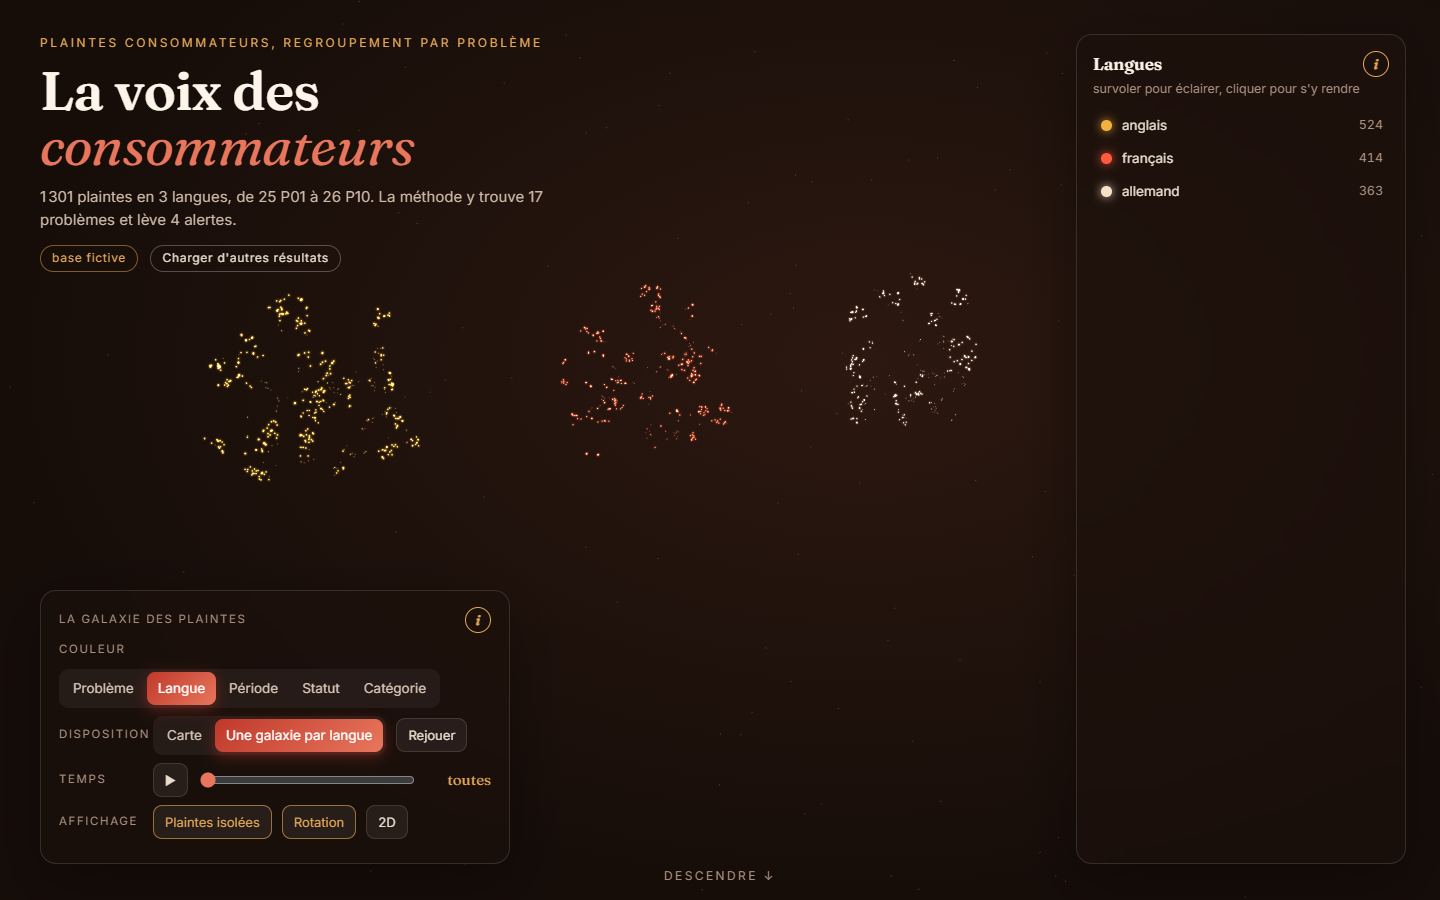
\includegraphics[width=\linewidth]{tdb_3_galaxie_par_langue.png}\\[2pt]{\footnotesize\textbf{Une galaxie par langue} : les mêmes amas reviennent dans chaque langue, donc les problèmes traversent les langues.}\end{tcolorbox}
\begin{tcolorbox}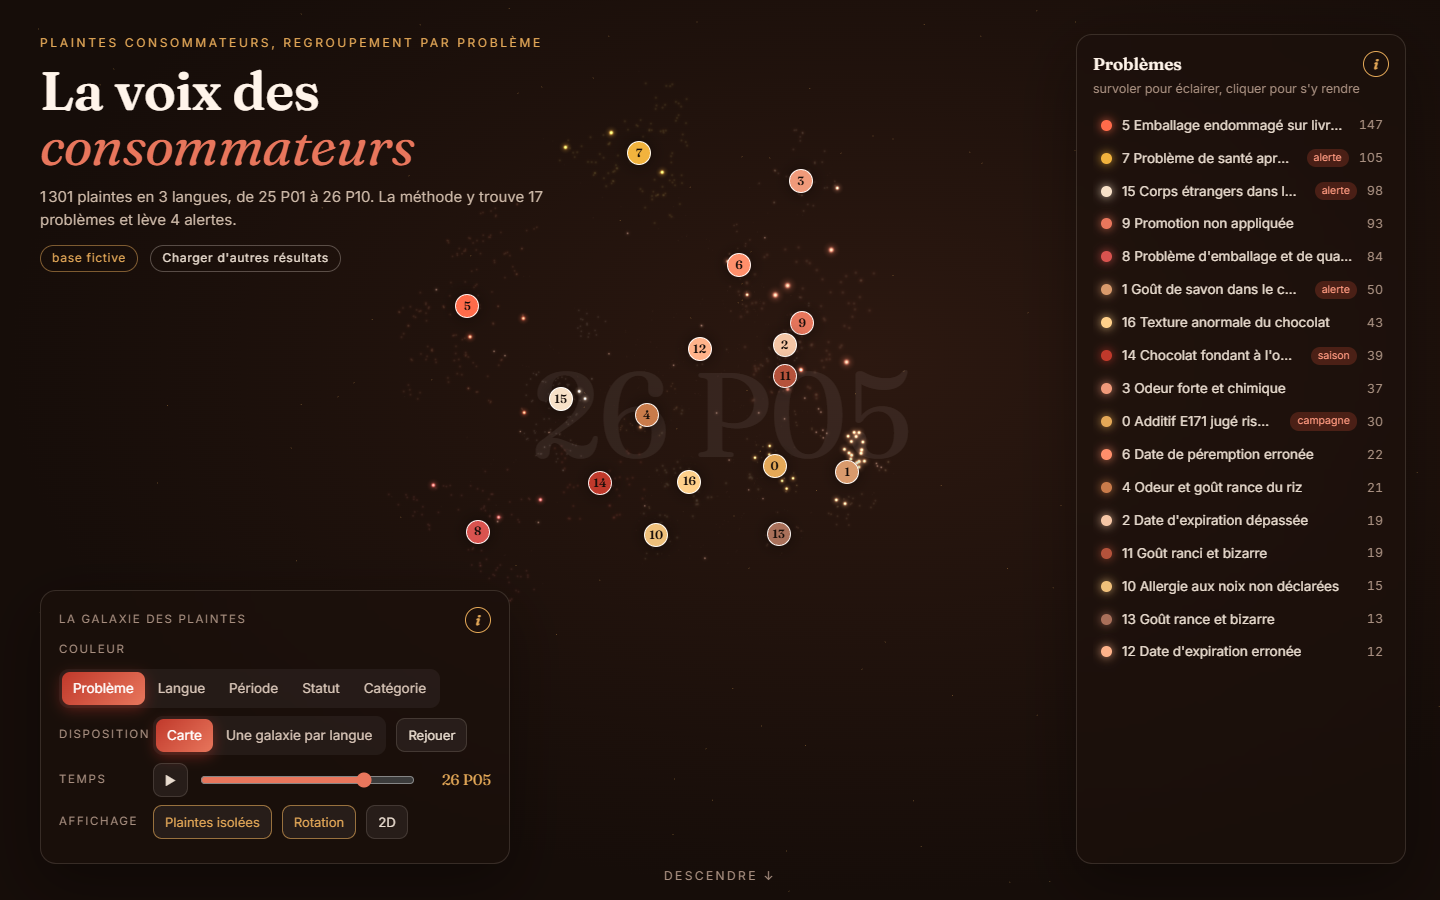
\includegraphics[width=\linewidth]{tdb_4_galaxie_periode.png}\\[2pt]{\footnotesize\textbf{Le temps} : le bouton \faPlay{} n'allume que les plaintes d'une période ; un amas qui s'allume d'un coup est un problème qui surgit.}\end{tcolorbox}
\begin{tcolorbox}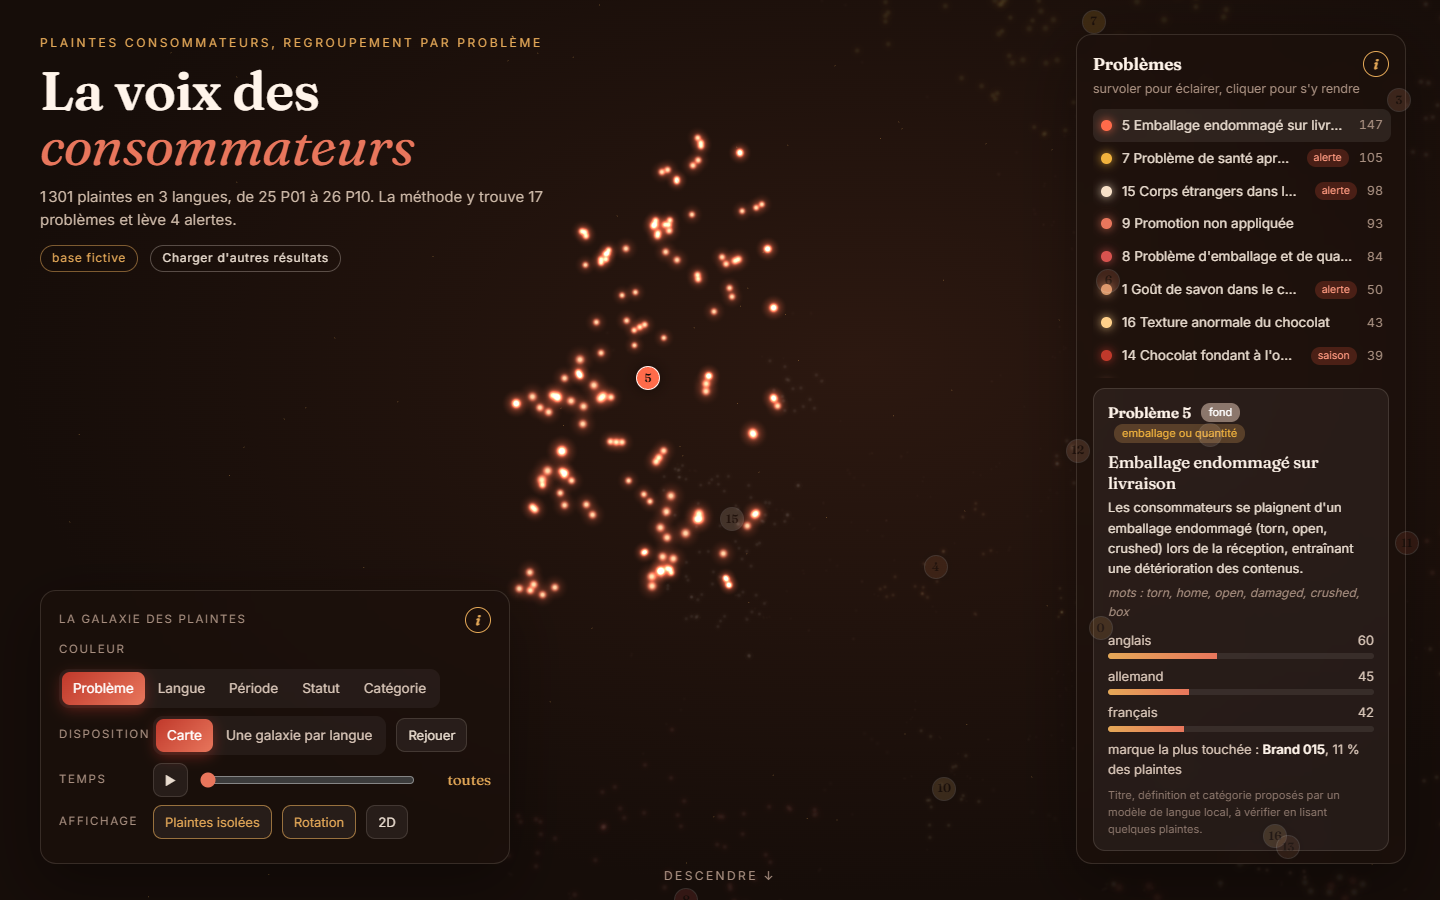
\includegraphics[width=\linewidth]{tdb_5_galaxie_focus.png}\\[2pt]{\footnotesize\textbf{Un clic sur un problème} : la caméra vole jusqu'à lui et sa fiche s'affiche (langues, marque la plus touchée, statut).}\end{tcolorbox}
\begin{tcolorbox}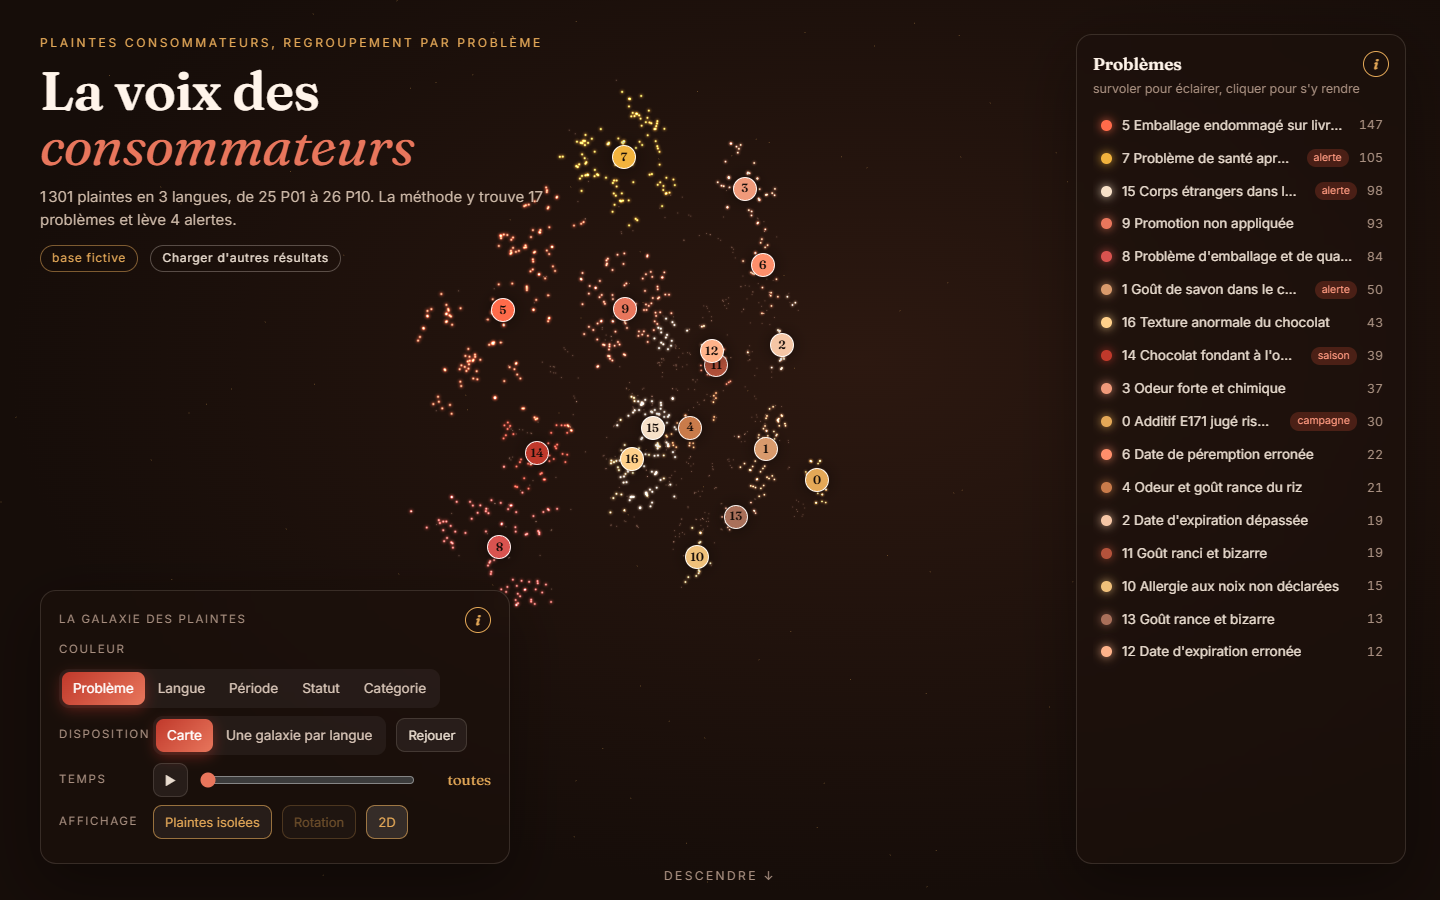
\includegraphics[width=\linewidth]{tdb_14_galaxie_2d.png}\\[2pt]{\footnotesize\textbf{Le bouton 2D} aplatit la galaxie pour la regarder de face.}\end{tcolorbox}
\begin{tcolorbox}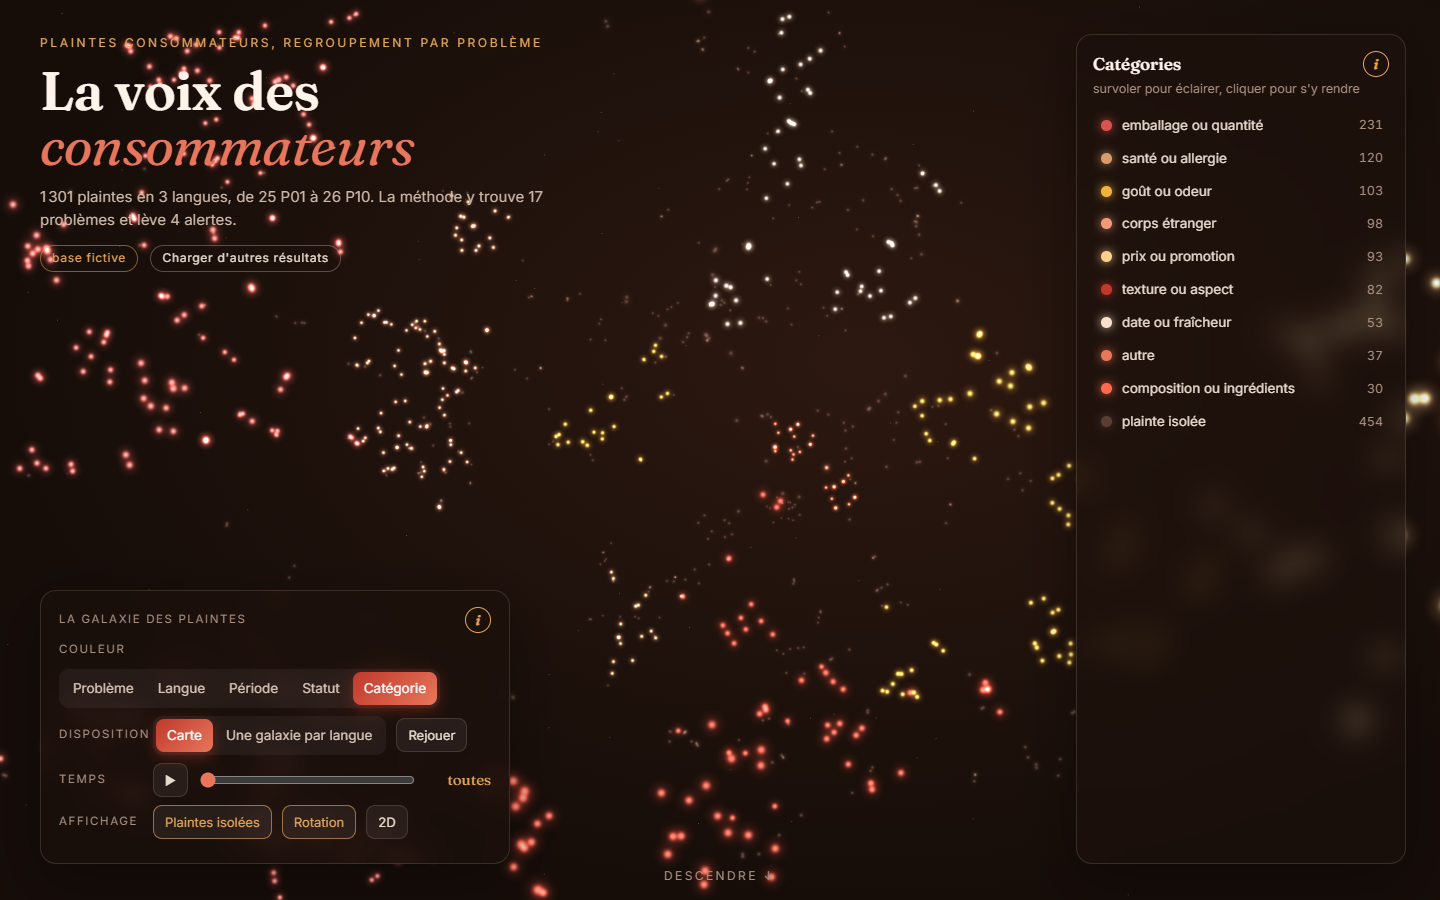
\includegraphics[width=\linewidth]{tdb_categorie_demo.png}\\[2pt]{\footnotesize\textbf{Le mode Catégorie} (base fictive) : chaque plainte prend la couleur de la famille de son problème, proposée par le modèle de langue local.}\end{tcolorbox}
\begin{tcolorbox}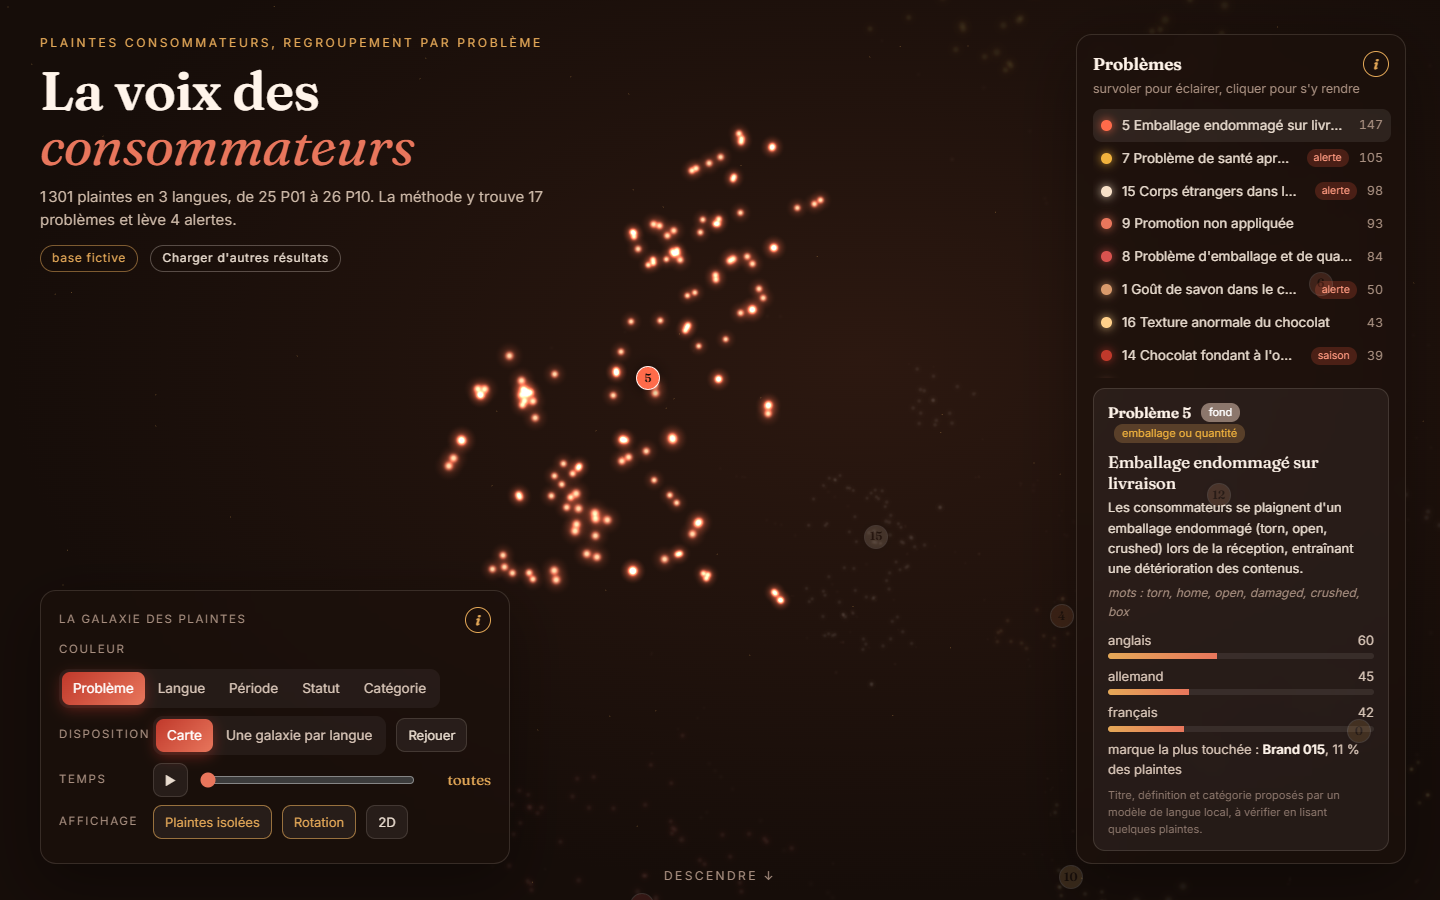
\includegraphics[width=\linewidth]{tdb_fiche_demo.png}\\[2pt]{\footnotesize\textbf{La fiche d'un problème} (base fictive) : titre, définition et catégorie proposés par le modèle de langue local, puis mots, langues, marque.}\end{tcolorbox}
\end{tcbraster}

\illus[0.98\linewidth]{tdb_8_relief.png}{Le relief des excès : chaque tour est une case problème $\times$ période.}

\begin{lire}
\textbf{Comment lire le relief.} La hauteur et la couleur disent combien de plaintes il y a eu par
rapport à ce qu'on attendait. Un problème normal a des tours plates ; une ou deux tours qui jaillissent
sur une ligne signalent un incident, une saison ou une campagne. Les tours rouge vif sont les alertes.
Le bouton \og À plat \fg{} montre la même chose en carte de chaleur.
\end{lire}

\illus[0.98\linewidth]{tdb_9_alertes.png}{Les cartes d'alerte, puis ce qui n'est pas un incident (saison, campagne).}

\begin{lire}
\textbf{Comment lire une carte d'alerte.} Le grand nombre : les plaintes de cette marque, pour ce
problème, à cette période ; à côté, combien on en attendait, et le rapport (\og $\times 16$ \fg{} : seize
fois plus). La phrase dit quelle part du pic porte la marque et quelle est la chance que ce soit le
hasard. Les petites barres reprennent la figure 5 du notebook.
\end{lire}

\begin{tcbraster}[raster columns=2, raster column skip=8pt, raster every box/.style={unbreakable, colback=white, colframe=palblue, boxrule=0.6pt, arc=4pt, left=3pt, right=3pt, top=3pt, bottom=3pt}]
\begin{tcolorbox}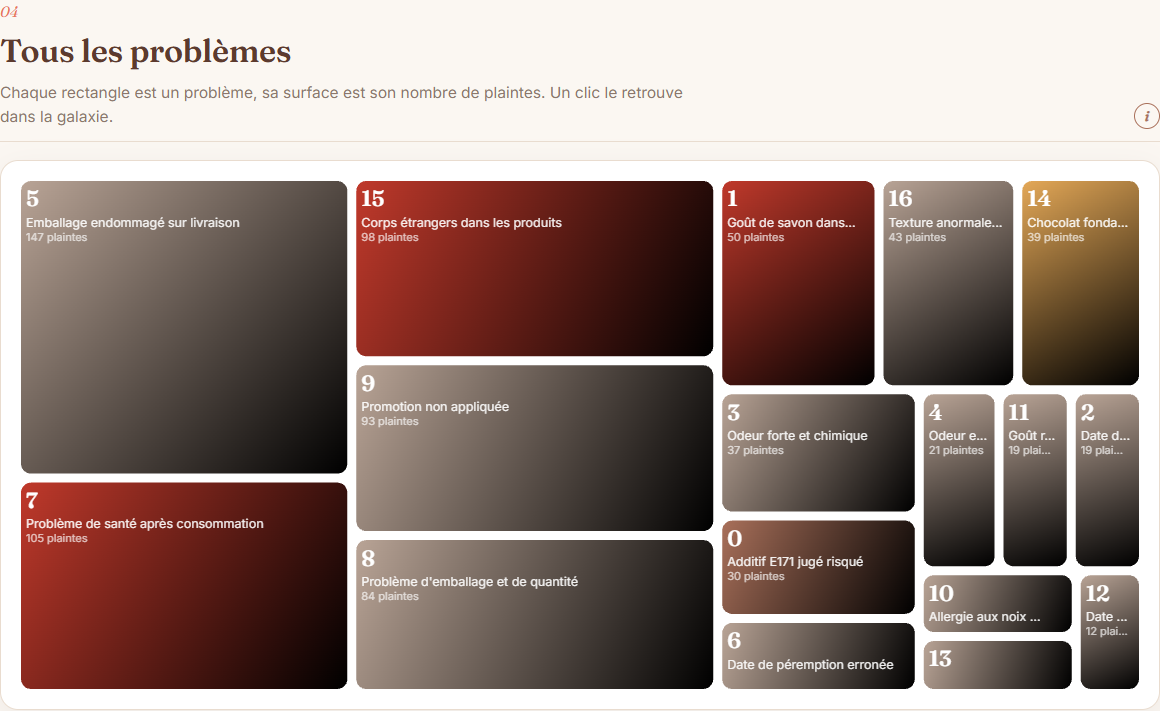
\includegraphics[width=\linewidth]{tdb_10_problemes.png}\\[2pt]{\footnotesize\textbf{La mosaïque} : un rectangle par problème, sa surface est son nombre de plaintes, sa couleur son statut. Un clic le retrouve dans la galaxie.}\end{tcolorbox}
\begin{tcolorbox}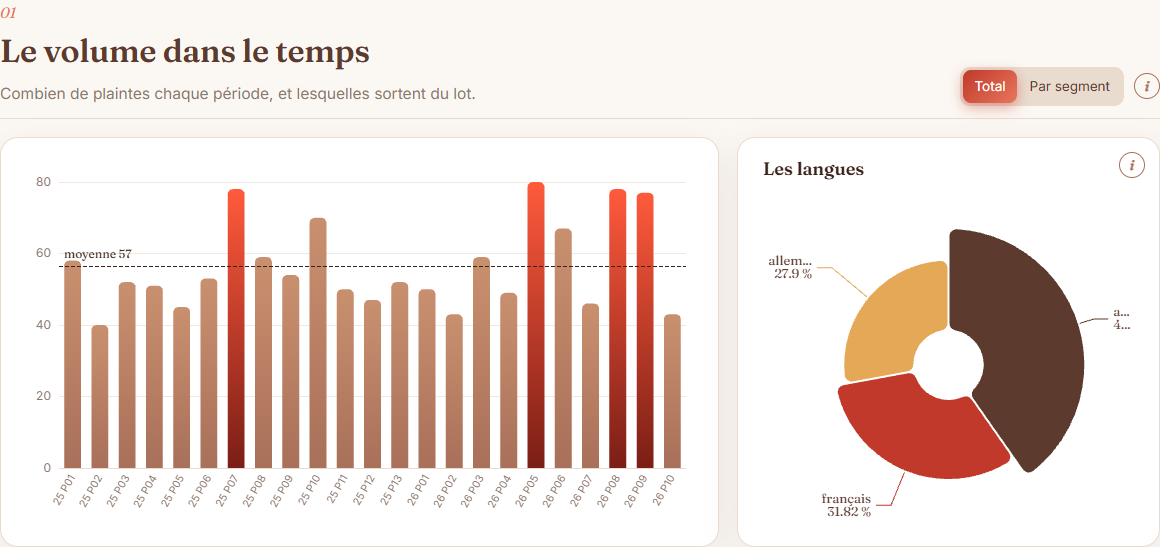
\includegraphics[width=\linewidth]{tdb_7_volume.png}\\[2pt]{\footnotesize\textbf{Le volume} par période, total ou par segment, avec les langues à côté.}\end{tcolorbox}
\begin{tcolorbox}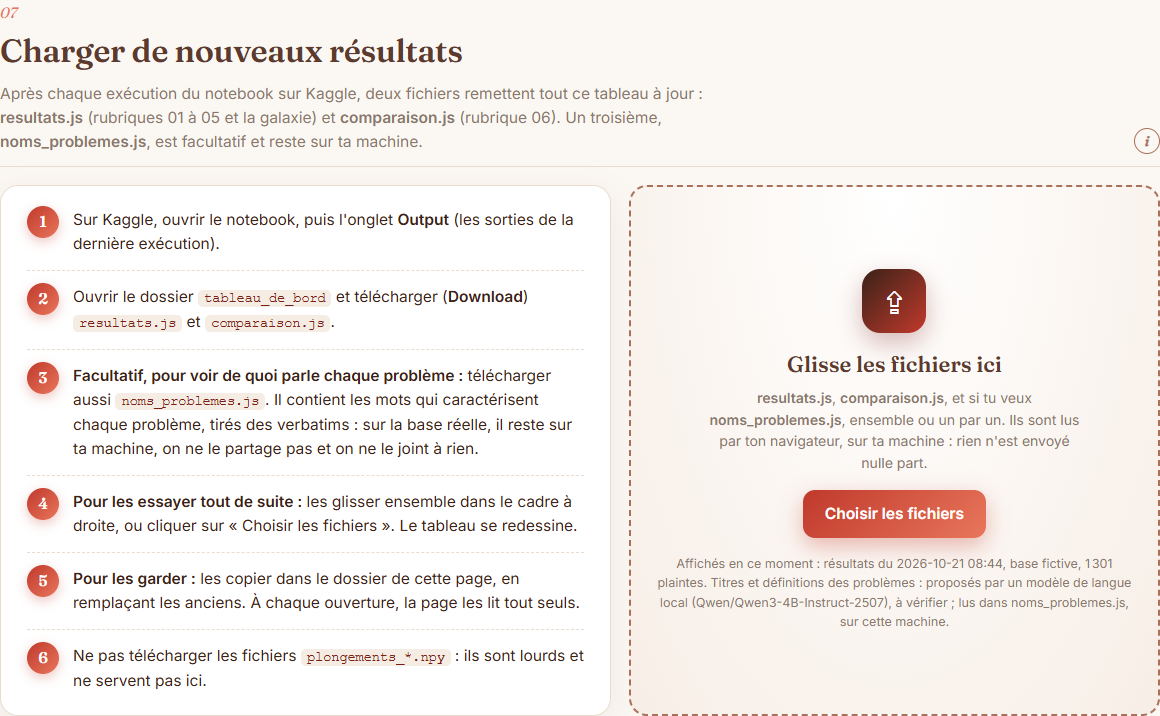
\includegraphics[width=\linewidth]{tdb_13_charger.png}\\[2pt]{\footnotesize\textbf{Charger de nouveaux résultats} : glisser les fichiers sur la page, ou les copier à côté d'elle.}\end{tcolorbox}
\end{tcbraster}

\illus[0.8\linewidth]{tdb_12_aide.png}{Le bouton \textit{i} : chaque graphique expliqué en quelques lignes.}

\bandeaupartie{II. La chaîne de comparaison}{La chaîne principale marche : on la rejoue avec huit outils, et on compare.}

\section{Avant de comparer : la chaîne principale est-elle validée ?}

\begin{stepbox}[title={7.0\quad Le bilan de la chaîne principale}]
La cellule 7.0 compte les vérifications \texttt{[OK]} de la chaîne principale, liste celles \texttt{[À revoir]}
et contrôle que \texttt{resultats.js} est écrit. \textbf{Lis chaque ligne \texttt{[À revoir]}} : ce n'est pas
forcément une erreur (une base sans incident ne lève aucune alerte), mais tu dois savoir l'expliquer.
\doisvoir{le nombre de vérifications réussies, la liste de celles à revoir, et \texttt{[OK]} pour \og la chaîne principale a écrit resultats.js \fg.}
\image{on goûte le plat avant d'acheter d'autres casseroles.}
\end{stepbox}

\begin{piege}
\textbf{Ne lance pas la comparaison sur une chaîne qui ne marche pas.} Si \texttt{resultats.js} n'est pas
écrit, reviens aux parties 0 à 6 : comparer huit outils sur une chaîne cassée ne dit rien de ces outils.
\end{piege}

\section{Partie 7 : comparer les outils}

La chaîne principale reste la même ; seule change la façon de transformer une plainte en vecteur.
Huit représentations, du comptage de mots à un transformer de 4 milliards de paramètres. Aucune
n'écrit de texte, et toutes tournent dans le notebook.

\begin{center}
\small
\renewcommand{\arraystretch}{1.22}
\rowcolors{2}{notebg}{white}
\begin{tabular}{@{}lllll@{}}
\rowcolor{titlebg}\color{white}\textbf{représentation} & \color{white}\textbf{origine} & \color{white}\textbf{type} & \color{white}\textbf{paramètres} & \color{white}\textbf{licence} \\
TF-IDF + SVD (100 dim.) & {\color{slate}\faFont}\ aucun créateur & comptage de mots & aucun & \\
MiniLM-L12 multilingue & \logo{sbert_logo}\logo{microsoft_logo} SBERT, Microsoft & transformer & 118 M & Apache 2.0 \\
e5-small multilingue & \logo{microsoft_logo} Microsoft & transformer & 118 M & MIT \\
e5-base multilingue & \logo{microsoft_logo} Microsoft & transformer & 278 M & MIT \\
e5-large multilingue & \logo{microsoft_logo} Microsoft & transformer & 560 M & MIT \\
BGE-M3 & \logo{baai_logo} BAAI & transformer & 568 M & MIT \\
\textbf{Qwen3-Embedding-0.6B} & \logo{qwen_logo} Alibaba (Qwen) & dérivé d'un LLM & 0,6 G & Apache 2.0 \\
Qwen3-Embedding-4B & \logo{qwen_logo} Alibaba (Qwen) & dérivé d'un LLM & 4 G & Apache 2.0 \\
\end{tabular}
\end{center}

% Copyright (c) 2026 Selina Cheggour. Tous droits réservés. Voir le fichier LICENSE.
% Tableau comparatif des modèles de plongement de la partie 7.
\subsection*{Tableau comparatif des modèles de plongement}

Les sept transformers de la partie~7 vont du modèle ultra-léger au modèle de plongement dérivé d'un LLM.
Les chiffres sont ceux des versions \textbf{multilingues} utilisées dans le notebook ; les versions
anglaises de MiniLM-L12 et de e5 sont plus petites (33, 110 et 335 M de paramètres).

\begin{center}
\scriptsize
\renewcommand{\arraystretch}{1.3}
\setlength{\tabcolsep}{2.5pt}
\rowcolors{2}{notebg}{white}
\begin{tabular}{@{}>{\raggedright\arraybackslash}p{2.1cm}>{\raggedright\arraybackslash}p{1.75cm}>{\raggedleft\arraybackslash}p{0.92cm}>{\raggedleft\arraybackslash}p{1.45cm}>{\raggedleft\arraybackslash}p{0.95cm}>{\raggedright\arraybackslash}p{4.18cm}>{\raggedright\arraybackslash}p{3.85cm}@{}}
\rowcolor{titlebg}\color{white}\textbf{modèle} & \color{white}\textbf{créateur} & \color{white}\textbf{param.} &
\color{white}\textbf{dim.} & \color{white}\textbf{jetons max} & \color{white}\textbf{points forts} &
\color{white}\textbf{usage idéal} \\
MiniLM-L12 multilingue & \logo{microsoft_logo}\logo{sbert_logo}\newline Microsoft, adapté par SBERT & 118 M & 384 & 128 &
Ultra-rapide, très peu gourmand, tourne sur processeur. &
Application légère, calcul en temps réel, petit budget d'infrastructure. \\
e5-small multilingue & \logo{microsoft_logo}\newline Microsoft & 118 M & 384 & 512 &
Rapide, bon rapport précision et vitesse, avec les préfixes \texttt{query:} et \texttt{passage:}. &
Prototype de RAG, moteur de recherche simple sur serveur léger. \\
e5-base multilingue & \logo{microsoft_logo}\newline Microsoft & 278 M & 768 & 512 &
Équilibré et polyvalent, meilleure finesse sémantique. &
Production standard, bon compromis entre coût et précision. \\
e5-large multilingue & \logo{microsoft_logo}\newline Microsoft & 560 M & 1\,024 & 512 &
Haute précision sémantique, capte bien les nuances. &
Recherche documentaire où la précision prime sur la vitesse. \\
BGE-M3 & \logo{baai_logo}\newline BAAI (Beijing Academy of AI) & 568 M & 1\,024 & 8\,192 &
Hybride, trois en un : dense, mots-clés (creux) et multi-vecteur (ColBERT). &
RAG sur documents longs qui demande à la fois le sens et les mots-clés exacts. \\
Qwen3-Embedding-0.6B (le modèle du TP) & \logo{qwen_logo}\newline Alibaba (Qwen) & 0,6 G & 1\,024 (32 à 1\,024, MRL) & 32\,768 &
Dérivé d'un LLM, sensible aux consignes, grande fenêtre de texte. &
RAG moderne sur textes longs, code, multilingue exigeant. \\
Qwen3-Embedding-4B & \logo{qwen_logo}\newline Alibaba (Qwen) & 4 G & 2\,560 (32 à 2\,560, MRL) & 32\,768 &
Parmi les meilleurs du classement MTEB multilingue à sa sortie (2025). &
Projet critique de très haute fidélité, avec une carte graphique dédiée. \\
\end{tabular}
\end{center}

\noindent{\footnotesize \textbf{param.} : nombre de paramètres. \textbf{dim.} : taille du vecteur produit.
\textbf{jetons max} : longueur maximale d'un texte, en jetons, au-delà de laquelle il est coupé.
\textbf{MRL} (\emph{Matryoshka Representation Learning}) : on peut ne garder que les premières coordonnées
du vecteur et perdre peu de qualité.\par}

\begin{notebox}[title={\faLightbulb\ Ce qu'il faut retenir pour choisir}]
\begin{itemize}[leftmargin=1.2em, itemsep=2pt]
\item Ultra-vitesse, sans carte graphique : MiniLM-L12 ou e5-small.
\item Un standard solide pour des textes courts ou moyens : e5-base ou e5-large.
\item Retrouver des mots-clés exacts (codes, références) dans des textes longs : BGE-M3.
\item Traiter de très longs documents (des PDF entiers) ou du code : Qwen3-Embedding (0.6B ou 4B).
\end{itemize}
Les plaintes du TP sont courtes et multilingues : c'est la mesure de la partie~7, pas ce tableau, qui
départage les modèles sur ces données.
\end{notebox}


\begin{stepbox}[title={7.1 à 7.4\quad Mesurer chaque modèle, à chaîne égale}]
\texttt{chaine(E)} reprend centrage, réglage automatique (3.3), regroupement, fusion et alertes,
sans graphiques. Pour chaque modèle on mesure :
\begin{formulabox}
\textbf{le temps} : $t^{\mathrm{ch}}$, chargement du modèle (téléchargement compris la première fois),
et $t^{\mathrm{calc}}$, calcul des $N$ vecteurs ; d'où $\tau = 1\,000\, t^{\mathrm{calc}} / N$, les secondes
pour 1\,000 plaintes.\\[3pt]
\textbf{la mémoire} : le maximum occupé sur la carte graphique.\\[3pt]
\textbf{le coût} pour $N'$ plaintes, avec un tarif horaire $p$ de la carte :
\[
c(N') = \frac{t^{\mathrm{ch}} + \tau\, N' / 1\,000}{3\,600} \times p .
\]
Kaggle est gratuit : $c$ est ce que coûterait la même carte louée. On suppose que le calcul croît comme
le nombre de plaintes.\\[3pt]
\textbf{la qualité} : la stabilité (ARI entre trois tirages de 90 \% des plaintes), le nombre de
problèmes et les alertes.
\end{formulabox}
\doisvoir{au moins cinq représentations mesurées, le TF-IDF compris, des temps positifs ; le fichier \texttt{comparaison.js} écrit, sans numéro de cas ni verbatim.}
\end{stepbox}

\illus[0.95\linewidth]{ill_comparaison_ari.png}{Base fictive, deux exécutions : avec les réglages fixes de 3.1 et 3.2, puis avec le réglage automatique de 3.3.}

\begin{lire}
\textbf{Comment lire ce graphique.} Une ligne par modèle. Le point cacao est l'accord avec les groupes
cachés quand tous les modèles ont les réglages choisis pour le modèle du TP ; le point rouge, quand chaque
modèle reçoit son propre réglage automatique. À droite, le nombre de problèmes trouvés dans les deux cas.
Plus le point est à droite, plus les problèmes trouvés coïncident avec les groupes cachés.
\end{lire}

\begin{questionbox}
\textbf{\faComments\ À discuter en équipe.} Avec les réglages fixes, cinq modèles réunissent presque tout
en 2 problèmes. Que vaut alors leur rappel, et pourquoi ce chiffre est-il trompeur ? Avec le réglage
automatique, certains modèles gagnent beaucoup, et le modèle du TP perd un peu : que mesure exactement la
règle de choix, et qu'est-ce qu'elle ne mesure pas ?
\end{questionbox}

\illus[0.86\linewidth]{tdb_15_outils.png}{Rubrique 06 du tableau de bord sur la base fictive, première exécution (réglages fixes).}

\begin{lire}
\textbf{Comment lire la rubrique 06.} Le podium donne le modèle le plus juste, le transformer le plus
rapide et la place du modèle du TP. Dans \og Qualité contre vitesse \fg, chaque bulle est un modèle
(taille : son nombre de paramètres) ; les bons choix sont en haut à gauche. Le temps sépare chargement et
calcul ; le coût se recalcule quand on change le tarif ou le nombre de plaintes ; la mémoire montre la
limite de 16 Go d'une carte T4.
\end{lire}

%%%%%%%%%%%%%%%%%%%%%%%%%%%%%%%%%%%%%%%%%%%%%%%%%%%%%%%%%%%%%%%%%%%%%%%%%%%%%%%%%%%%%%%%%%%%%%%%%%%%%%%%
\section{Partie 8 : ce qui peut sortir de Kaggle}

\begin{center}
\begin{tikzpicture}[
  num/.style={circle,fill=accentblue,text=white,font=\bfseries\Large,minimum size=0.9cm},
  lab/.style={align=center,font=\small,text width=4.2cm},
  arr/.style={-{Stealth[length=3mm]},very thick,color=accentblue}]
\node[num] (n1) {1}; \node[num,right=4.2cm of n1] (n2) {2}; \node[num,right=4.2cm of n2] (n3) {3};
\node[lab,below=2pt of n1] {\textbf{Add Input} : le jeu de données \textbf{privé} de la base réelle};
\node[lab,below=2pt of n2] {cellule 0.1 : le nom du fichier est déjà écrit, rien à modifier};
\node[lab,below=2pt of n3] {tout exécuter : aucun verbatim ne s'affiche};
\draw[arr] (n1) -- (n2); \draw[arr] (n2) -- (n3);
\end{tikzpicture}
\end{center}

\begin{tcbraster}[raster columns=2, raster equal height, raster column skip=8pt]
\begin{card}{sectioncolor}{\faSignOut*\ Ce qui peut sortir de Kaggle}
\begin{itemize}[leftmargin=1.3em,itemsep=2pt]
\item[\faCheck] le rapport de lecture, les comptes par langue, marque, période
\item[\faCheck] le nombre et la taille des groupes, la stabilité
\item[\faCheck] les cases anormales (numéro du problème, marque, période, observé, attendu, $q$)
\item[\faCheck] \texttt{resultats.js} et \texttt{comparaison.js}
\end{itemize}
\end{card}
\begin{card}{slate}{\faBan\ Ce qui ne sort pas}
\begin{itemize}[leftmargin=1.3em,itemsep=2pt]
\item[\faTimes] les verbatims et les numéros de cas
\item[\faTimes] les vecteurs \texttt{plongements\_*.npy}
\item[\faTimes] les mots et définitions des problèmes, sauf accord écrit de l'entreprise
\item[\faTimes] les figures 3 à 5, dont les légendes sont faites de ces mots
\end{itemize}
\end{card}
\end{tcbraster}

\begin{piege}
\textbf{Sur de vraies plaintes, des réglages trouvés ailleurs ne tiennent pas forcément.} Les
vraies lettres sont plus longues, plus variées, et peuvent contenir une grosse campagne. C'est exactement
pour cela que l'exercice 3.3 choisit le réglage sur les données elles-mêmes, avec un plan B.
\end{piege}

% Copyright (c) 2026 Selina Cheggour. Tous droits réservés. Voir le fichier LICENSE.
% Lexique simple et pistes pour aller plus loin.

\bandeaupartie{Lexique et pistes}{Les mots du TP, en une phrase chacun ; puis ce qu'on pourrait faire ensuite.}

\section{Lexique}

\renewcommand{\arraystretch}{1.32}
\rowcolors{2}{notebg}{white}
\begin{tabularx}{\linewidth}{>{\bfseries\leavevmode\color{darkblue}}p{3.7cm}X}
\rowcolor{titlebg}\color{white}mot & \leavevmode\color{white}\textbf{en une phrase} \\
verbatim & le texte libre écrit par le consommateur, tel qu'il est arrivé. \\
apprentissage non supervisé & on cherche une structure dans des données sans étiquette : ici, des groupes de plaintes. \\
TF-IDF & une coordonnée par mot ; un mot pèse lourd s'il est fréquent dans la plainte et rare ailleurs. \\
cosinus & la proximité de deux vecteurs : 1 s'ils pointent dans la même direction, 0 s'ils n'ont rien en commun. \\
jeton & le morceau de texte que lit un transformer : un mot fréquent, ou un bout de mot rare. \\
transformer & un réseau de neurones où chaque jeton \og regarde \fg{} tous les autres (l'attention) pour préciser son sens. \\
plongement & le vecteur de sens qu'un transformer donne à un texte entier. \\
centrage par langue & retirer à chaque vecteur la moyenne de sa langue, pour ne garder que ce que la plainte dit. \\
t-SNE & une méthode qui dessine en 2 ou 3 dimensions des points proches dans un grand espace ; les axes n'ont pas de sens. \\
ACP & l'analyse en composantes principales : garder les quelques directions où les données varient le plus. \\
HDBSCAN & un regroupement par densité, qui trouve seul le nombre de groupes et laisse de côté les points isolés. \\
Ward & une classification hiérarchique qui range chaque point, en fusionnant les groupes qui augmentent le moins la dispersion. \\
groupes jumeaux & le même problème trouvé deux fois, une fois par langue. \\
\end{tabularx}

\begin{tabularx}{\linewidth}{>{\bfseries\leavevmode\color{darkblue}}p{3.7cm}X}
\rowcolor{titlebg}\color{white}mot & \leavevmode\color{white}\textbf{en une phrase (suite)} \\
c-TF-IDF & le TF-IDF calculé sur un groupe entier, pour trouver ses mots les plus caractéristiques. \\
LLM & un grand modèle de langue qui écrit du texte ; ici, il tourne dans le notebook et propose titres et définitions. \\
ARI & l'indice de Rand ajusté : l'accord entre deux regroupements, 1 s'ils sont identiques, 0 au hasard. \\
loi de Poisson & la loi du nombre d'événements rares quand on en attend en moyenne $\lambda$. \\
p-valeur & la probabilité d'observer au moins autant si le hasard seul jouait. \\
Benjamini-Hochberg & une correction des p-valeurs quand on fait beaucoup de tests à la fois. \\
part dans le pic & la part des plaintes d'un problème, sur une période, qui vient d'une seule marque. \\
quasi doublon & une plainte dont la plus proche voisine TF-IDF a un cosinus supérieur à 0,9. \\
incident candidat & un problème en excès sur une marque et une période, porté surtout par cette marque. \\
pic partagé & un problème en excès sur une période chez plusieurs marques à la fois. \\
campagne & un groupe de messages presque identiques : une mobilisation, pas un défaut. \\
rappel, précision & la part d'un groupe caché retrouvée ensemble ; la part d'un groupe trouvé qui vient du groupe caché. \\
\end{tabularx}

\clearpage
\section{Pour aller plus loin}

\begin{tcbraster}[raster columns=2, raster equal height, raster column skip=8pt, raster row skip=8pt]
\begin{conceptbox}[title={\faLanguage\ Traduire avant de comparer}, unbreakable]
\small Au lieu de centrer par langue, traduire toutes les plaintes dans une seule langue avec un modèle de
traduction qui tourne dans le notebook. Plus lourd, mais sans le risque de retirer une partie du sens avec
la langue.
\end{conceptbox}
\begin{conceptbox}[title={\faCalendar*\ La date de l'événement}, unbreakable]
\small Une plainte peut arriver des semaines après l'achat. Si l'entreprise fournit la date de fabrication
ou le numéro de lot, l'alerte pourrait porter sur le lot plutôt que sur la période de la plainte.
\end{conceptbox}
\begin{conceptbox}[title={\faStore\ D'autres cases que la marque}, unbreakable]
\small Quand une marque domine la base, comparer les marques n'a plus de sens : on peut tester l'excès par
segment, par pays (si la colonne existe), ou par période seule.
\end{conceptbox}
\begin{conceptbox}[title={\faUserCheck\ Une évaluation humaine}, unbreakable]
\small Faire relire, par une personne habilitée, quelques plaintes de chaque problème et noter si le titre
proposé par le LLM est juste : c'est la seule façon de mesurer la qualité sur la base réelle.
\end{conceptbox}
\begin{conceptbox}[title={\faProjectDiagram\ D'autres regroupements}, unbreakable]
\small Réduire les vecteurs avec UMAP avant HDBSCAN, ou essayer une modélisation de sujets complète
(BERTopic), et les ajouter à la chaîne de comparaison, à côté des huit outils.
\end{conceptbox}
\begin{conceptbox}[title={\faBell\ Une alerte au fil de l'eau}, unbreakable]
\small Recalculer chaque semaine les cases anormales sur les nouvelles plaintes seulement, et n'alerter
que sur ce qui change : c'est ainsi qu'un tel outil servirait au quotidien.
\end{conceptbox}
\end{tcbraster}

\vfill
\begin{center}\color{slate}\small
\faUserTie\quad Une question ? Lève la main, l'encadrante passe.
\end{center}

% Copyright (c) 2026 Selina Cheggour. Tous droits réservés. Voir le fichier LICENSE.
% Annexe : les outils expliqués (babel, py3langid, expressions régulières et nettoyage, centrage par langue).

\bandeaupartie{Annexe : les outils expliqués}{babel, py3langid, les expressions régulières du nettoyage,\\et le centrage par langue expliqué avec des notes de classe.}

\section{babel : le nom des langues en clair}

\begin{stepbox}[title={\faLanguage\quad Ce que c'est}]
\texttt{babel} est une bibliothèque Python d'\textbf{internationalisation} : pour chaque langue d'affichage,
elle connaît les noms des langues et des pays, les formats de dates, de nombres et de monnaies. Elle les
tire du \textbf{CLDR} (\emph{Common Locale Data Repository}), la base de référence du consortium Unicode,
celle qu'utilisent aussi les navigateurs et les systèmes d'exploitation.
\end{stepbox}

\begin{stepbox}[title={\faCogs\quad Ce qu'elle fait dans le notebook}]
Une seule chose : écrire en clair le nom des langues détectées. Le détecteur de langue (ci-dessous) ne
renvoie qu'un \textbf{code}, comme \texttt{fr}, \texttt{nl} ou \texttt{ary}. babel le traduit en nom
français :
\begin{lstlisting}[escapeinside={(*}{*)}]
from babel import Locale
NOMS_CLDR = Locale("fr").languages      # un dictionnaire : code -> nom en français
NOMS_CLDR["nl"]                          # 'néerlandais'
NOMS_CLDR["ary"]                         # 'arabe marocain'
\end{lstlisting}
Quelques codes rares que le CLDR ne nomme pas sont complétés à la main dans \texttt{COMPLEMENT\_LANGUES}
(par exemple \texttt{zxx}, \og sans contenu linguistique \fg). Le nom affiché est donc, dans l'ordre : le
complément s'il existe, sinon le nom donné par babel, sinon le code lui-même.
\end{stepbox}

\begin{tcbraster}[raster columns=2, raster equal height, raster column skip=8pt, raster every box/.style={unbreakable}]
\begin{conceptbox}[title={\faDownload\ Installée en 0.2}, unbreakable]
\small Elle n'est pas dans l'image Kaggle par défaut : la cellule 0.2 l'installe avec \texttt{py3langid}.
Si elle manque, rien ne plante : les langues s'affichent par leur code.
\end{conceptbox}
\begin{conceptbox}[title={\faLock\ Ne touche pas aux plaintes}, unbreakable]
\small Elle ne lit aucun texte et n'envoie rien sur internet. Elle ne joue aucun rôle dans les vecteurs, les
groupes ou les alertes : elle sert seulement à l'affichage.
\end{conceptbox}
\end{tcbraster}

%%%%%%%%%%%%%%%%%%%%%%%%%%%%%%%%%%%%%%%%%%%%%%%%%%%%%%%%%%%%%%%%%%%%%%%%%%%%%%%%%%%%%%%%%%%%%%%%%%%%%%%%
\section{py3langid : quelle langue pour chaque plainte}

\begin{stepbox}[title={\faSearch\quad Ce que c'est}]
\texttt{py3langid} est un \textbf{détecteur de langue} : on lui donne un texte, il renvoie le code de la
langue la plus probable. C'est la version modernisée de \texttt{langid.py}. Son modèle, un petit modèle
probabiliste (Bayes naïf), a appris sur des textes de plus d'une centaine de langues quelles
\textbf{suites de caractères} sont typiques de chacune : \og ijk \fg{} en néerlandais, \og sch \fg{} en
allemand, \og eau \fg{} en français. Il est livré avec le paquet et tourne sur le processeur, sans internet
et sans carte graphique, en une fraction de seconde pour toute la base.
\end{stepbox}

\begin{stepbox}[title={\faCogs\quad Ce qu'il fait dans le notebook (exercice 1.4)}]
\begin{lstlisting}[escapeinside={(*}{*)}]
import py3langid
py3langid.classify("Bonjour, le chocolat avait un go(*\^u*)t de savon.")
# ('fr', -209.3)  : le code de la langue, puis un score
plaintes["langue"] = [py3langid.classify(t)[0] if t else "?" for t in plaintes.texte]
\end{lstlisting}
\texttt{classify} renvoie deux valeurs ; on garde la première, le code (\texttt{[0]}). Le score est une
\textbf{log-probabilité} : plus il est grand, plus le modèle est sûr, mais ce n'est pas un pourcentage. Un
texte vide reçoit \texttt{"?"}.
\doisvoir{une langue pour chaque plainte, et une répartition avec quelques langues principales.}
\end{stepbox}

\begin{piege}
\textbf{La langue n'est pas le pays.} L'anglais, le français et l'allemand couvrent chacun plusieurs pays.
\textbf{Et le détecteur se trompe sur les textes très courts} ou pleins de chiffres et de références : une
langue qui ne compte qu'une ou deux plaintes est souvent une erreur de détection, pas un vrai pays de plus.
\end{piege}

%%%%%%%%%%%%%%%%%%%%%%%%%%%%%%%%%%%%%%%%%%%%%%%%%%%%%%%%%%%%%%%%%%%%%%%%%%%%%%%%%%%%%%%%%%%%%%%%%%%%%%%%
\section{Les expressions régulières du nettoyage (exercice 1.2)}

\subsection{re, c'est quoi ?}

\texttt{re} est le module de Python pour les \textbf{expressions régulières} (\emph{regular expressions}).
Une expression régulière est un \textbf{motif} qui décrit une \emph{forme} de texte, au lieu d'un texte
exact. Au lieu de chercher le lien précis \texttt{https://exemple.io}, on décrit la forme de tous les liens :
\og commence par http, peut-être un s, puis ://, puis des caractères sans espace \fg.

\subsection{Comment se lit re.sub}

\texttt{re.sub} veut dire \emph{substitute}, remplacer. Elle prend toujours trois choses, dans cet ordre :
\begin{center}
\begin{tikzpicture}[b/.style={draw=#1, fill=#1!10, rounded corners=4pt, font=\small, align=center, minimum height=1cm, text width=3.6cm}]
\node[b=sectioncolor] (m) {\textbf{1. le motif}\\ce qu'on cherche};
\node[b=accentblue, right=0.4cm of m] (r) {\textbf{2. le remplacement}\\par quoi on le remplace};
\node[b=darkblue, right=0.4cm of r] (t) {\textbf{3. le texte}\\où on cherche};
\node[above=0.15cm of r, font=\ttfamily\small] {re.sub( motif , remplacement , texte )};
\end{tikzpicture}
\end{center}
Elle renvoie le texte modifié. Exemple : \verb|re.sub(r"\*{2,}", " ", texte)| se lit \og dans
\texttt{texte}, remplace chaque suite de deux étoiles ou plus par une espace \fg.

\begin{tcbraster}[raster columns=2, raster equal height, raster column skip=8pt, raster every box/.style={unbreakable}]
\begin{conceptbox}[title={Le \texttt{r} devant le motif}, unbreakable]
\small \verb|r"..."| est un texte \og brut \fg{} : Python garde les barres \verb|\| telles quelles et les
passe au motif.
\end{conceptbox}
\begin{conceptbox}[title={\texttt{texte}, à la fin}, unbreakable]
\small C'est la variable qui contient la plainte à nettoyer. Le résultat de chaque ligne remplace
\texttt{texte}, et la ligne suivante repart de lui.
\end{conceptbox}
\end{tcbraster}

\subsection{Les briques pour lire les motifs}

\begin{center}
\renewcommand{\arraystretch}{1.3}
\rowcolors{2}{notebg}{white}
\begin{tabular}{@{}>{\centering\arraybackslash}p{2.2cm}p{11.8cm}@{}}
\rowcolor{titlebg}\color{white}\textbf{symbole} & \color{white}\textbf{veut dire} \\
\verb|^| & le tout début du texte \\
\verb|\s| & un \og blanc \fg{} : espace, tabulation, retour à la ligne \\
\verb|\S| & tout sauf un blanc \\
\verb|*| & 0 fois ou plus le symbole d'avant \\
\verb|+| & 1 fois ou plus le symbole d'avant \\
\verb|?| & 0 ou 1 fois le symbole d'avant : il est facultatif \\
\verb|{2,}| & 2 fois ou plus le symbole d'avant \\
\verb|\*| & une vraie étoile (la barre empêche de la lire comme \og 0 fois ou plus \fg) \\
\verb|[.!?]| & un seul caractère parmi ceux de la liste \\
\verb|[^\W\d_]| & une lettre, de n'importe quel alphabet (ni chiffre, ni ponctuation, ni \_) \\
\verb|(...)| et \verb|\1| & on capture un morceau, puis on le remet tel quel dans le remplacement \\
\verb|(?=...)| & regarde ce qui suit, sans le consommer ni le modifier \\
\end{tabular}
\end{center}

\subsection{Les cinq étapes de nettoyer, une par une}

\begin{lstlisting}[escapeinside={(*}{*)}]
def nettoyer(texte):
    texte = re.sub(r"^\s*EXTERNAL", "", texte)               # 1
    texte = re.sub(r"https?://\S+", " ", texte)               # 2
    texte = re.sub(r"\*{2,}", " ", texte)                     # 3
    texte = re.sub(r"([.!?;:,(*\textcolor{accentblue}{\textsf{\scriptsize virgule arabe}}*)])(?=[^\W\d_])", r"\1 ", texte) # 4
    return re.sub(r"\s+", " ", texte).strip()                 # 5
\end{lstlisting}

\begin{center}
\renewcommand{\arraystretch}{1.35}
\rowcolors{2}{notebg}{white}
\begin{tabular}{@{}>{\bfseries\color{sectioncolor}}c p{6.4cm}p{6.6cm}@{}}
\rowcolor{titlebg}\color{white}\# & \color{white}\textbf{ce que fait le motif} & \color{white}\textbf{exemple} \\
1 & au début du texte (\verb|^|), des blancs ou rien, puis le mot EXTERNAL : supprimé & \texttt{EXTERNALBonjour} $\to$ \texttt{Bonjour} \\
2 & \texttt{http}, un \texttt{s} facultatif, \texttt{://}, puis tout jusqu'au premier blanc : le lien entier devient une espace & \texttt{voir https://exemple.io/aB3} $\to$ \texttt{voir \textvisiblespace} \\
3 & deux étoiles ou plus (les produits masqués) : une espace & \texttt{acheté ******* hier} $\to$ \texttt{acheté \textvisiblespace\textvisiblespace\textvisiblespace hier} \\
4 & une ponctuation suivie directement d'une lettre : on garde la ponctuation (\verb|\1|) et on ajoute une espace & \texttt{Bonjour,J'ai} $\to$ \texttt{Bonjour, J'ai} ; \texttt{3.5} ne bouge pas \\
5 & les espaces simples : chaque groupe de blancs devient une seule espace, puis \texttt{.strip()} enlève les blancs du début et de la fin & \texttt{acheté \textvisiblespace\textvisiblespace\textvisiblespace hier} $\to$ \texttt{acheté hier} \\
\end{tabular}
\end{center}
{\small\color{slate}\textit{Le signe \textvisiblespace{} montre une espace.}}

\subsection{L'étape 5 et strip, en détail}

\begin{stepbox}[title={5\quad Des espaces simples}]
La dernière ligne fait deux choses, de gauche à droite.
\begin{enumerate}[nosep]
\item \verb|re.sub(r"\s+", " ", texte)| : \verb|\s+| veut dire \og un blanc ou plus, d'affilée \fg. Chaque
  groupe de blancs, qu'il compte 1 ou 10 espaces, tabulations ou retours à la ligne, devient \textbf{une
  seule espace}.
\item \texttt{.strip()} n'est pas du \texttt{re} : c'est une méthode de tout texte Python. Elle enlève les
  blancs au \textbf{début} et à la \textbf{fin}, jamais au milieu :
  \verb|"  Bonjour le monde  ".strip()| donne \verb|"Bonjour le monde"|.
\end{enumerate}
Cette étape est nécessaire parce que les étapes d'avant \textbf{créent} des espaces en trop :
\begin{lstlisting}[escapeinside={(*}{*)}]
départ      : "EXTERNALBonjour, j'ai acheté ******* hier"
après 1     : "Bonjour, j'ai acheté ******* hier"
après 3     : "Bonjour, j'ai acheté   hier"     (trois espaces)
après 5     : "Bonjour, j'ai acheté hier"       (une seule)
\end{lstlisting}
Un lien en fin de message devient lui aussi une espace finale, que \texttt{.strip()} retire.
\image{après avoir découpé des étiquettes dans une lettre, on referme les trous pour que le texte se lise d'une traite.}
\end{stepbox}

%%%%%%%%%%%%%%%%%%%%%%%%%%%%%%%%%%%%%%%%%%%%%%%%%%%%%%%%%%%%%%%%%%%%%%%%%%%%%%%%%%%%%%%%%%%%%%%%%%%%%%%%
\section{Le centrage par langue, avec des notes de classe (exercice 2.3)}

\subsection{Deux professeurs, deux façons de noter}

\begin{tcbraster}[raster columns=2, raster equal height, raster column skip=8pt, raster every box/.style={unbreakable}]
\begin{bloc}[sectioncolor]{\faUserTie\quad La classe du professeur dur}
\begin{center}
\renewcommand{\arraystretch}{1.2}
\rowcolors{2}{notebg}{white}
\begin{tabular}{lr}
\textbf{élève} & \textbf{note} \\
Ali & 6 \\
Bea & 8 \\
Chloé & 9 \\
Dan & 10 \\
\textbf{Léa} & \textbf{12} \\
\end{tabular}
\end{center}
Moyenne de la classe : $(6 + 8 + 9 + 10 + 12) / 5 = 45 / 5 = 9$.
\end{bloc}
\begin{bloc}[accentblue]{\faUserGraduate\quad La classe du professeur large}
\begin{center}
\renewcommand{\arraystretch}{1.2}
\rowcolors{2}{notebg}{white}
\begin{tabular}{lr}
\textbf{élève} & \textbf{note} \\
\textbf{Tom} & \textbf{12} \\
Uma & 14 \\
Vic & 15 \\
Wael & 16 \\
Zoé & 18 \\
\end{tabular}
\end{center}
Moyenne de la classe : $(12 + 14 + 15 + 16 + 18) / 5 = 75 / 5 = 15$.
\end{bloc}
\end{tcbraster}

\subsection{Même note, deux histoires opposées}

\begin{tcbraster}[raster columns=2, raster equal height, raster column skip=8pt, raster every box/.style={unbreakable}]
\begin{kpibox}[title={Léa : $12 - 9 = +3$}, unbreakable]
\small Léa a 3 points \textbf{de plus} que ce que son professeur donne d'habitude. C'est la
\textbf{meilleure} de sa classe.
\end{kpibox}
\begin{kpibox}[title={Tom : $12 - 15 = -3$}, unbreakable]
\small Tom a 3 points \textbf{de moins} que ce que son professeur donne d'habitude. C'est le
\textbf{dernier} de sa classe.
\end{kpibox}
\end{tcbraster}

Les deux ont 12. Le $+3$ et le $-3$ montrent la différence ; le 12 brut la cachait. Le
\textbf{centrage}, c'est juste ça : \textbf{remplacer la note par l'écart à la moyenne de son propre
professeur}. On ne compare plus des notes, on compare ce que chaque élève a de plus ou de moins que sa
classe.

\subsection{Le lien avec les plaintes}

\begin{center}
\renewcommand{\arraystretch}{1.35}
\rowcolors{2}{notebg}{white}
\begin{tabular}{@{}p{4.6cm}p{9.4cm}@{}}
\rowcolor{titlebg}\color{white}\textbf{dans la classe} & \color{white}\textbf{dans le notebook} \\
le professeur & la \textbf{langue} de la plainte \\
la note d'un élève & le \textbf{plongement} $\mathbf{e}_i$ de la plainte : 1\,024 nombres au lieu d'un seul \\
la moyenne de la classe & la moyenne $\boldsymbol{\mu}_\ell$ des plongements de toutes les plaintes de la langue $\ell$ \\
l'écart $+3$ ou $-3$ & $\mathbf{e}_i - \boldsymbol{\mu}_{\ell(i)}$ : ce que la plainte dit \textbf{de plus} que les autres plaintes de sa langue \\
\end{tabular}
\end{center}

Un plongement mélange deux choses : ce que dit la plainte (le sujet) et la façon dont sa langue
s'exprime (la \og façon de noter \fg{} du professeur). Deux plaintes allemandes sur des sujets différents
se ressemblent un peu, simplement parce qu'elles sont en allemand. En retirant à chaque plainte la
moyenne de sa langue, on retire cette part commune, et il reste le sujet : une plainte française et une
plainte allemande sur le goût de savon se retrouvent alors côte à côte.

\begin{tcbraster}[raster columns=2, raster equal height, raster column skip=8pt, raster every box/.style={unbreakable}]
\begin{conceptbox}[title={\faRulerCombined\ Puis on renorme}, unbreakable]
\small Après la soustraction, on divise par la longueur du vecteur (le dénominateur de la formule de
l'exercice 2.3), pour que toutes les plaintes aient la même longueur, 1.
\end{conceptbox}
\begin{conceptbox}[title={\faUsers\ Les petites classes}, unbreakable]
\small Une moyenne sur deux élèves ne dit rien du professeur. De même, une langue de moins de 10 plaintes
reçoit la moyenne de \textbf{toutes} les plaintes, pas la sienne.
\end{conceptbox}
\end{tcbraster}

% Annexe : cosinus, similarité et distance (exercices 2.1 et 3.2), en images.

\section{Cosinus : similarité et distance (exercices 2.1 et 3.2)}

\subsection{Le cosinus regarde l'angle entre deux flèches}

Chaque plainte, et chaque centre de groupe, est une \textbf{flèche} (un vecteur). Le \textbf{cosinus} ne
regarde pas la longueur des flèches, seulement l'\textbf{angle} entre elles : il dit si elles pointent dans
la même direction, donc si les deux textes parlent de la même chose.

\begin{center}
\begin{tikzpicture}[fl/.style={-{Stealth[length=3mm]}, line width=1.6pt}]
\foreach \dx/\ang/\cosv/\dv/\titre/\coul in {0/8/1/0/même direction/accentblue, 5.4/60/0{,}5/0{,}5/à moitié/ambre, 10.8/90/0/1/rien en commun/slate} {
  \begin{scope}[xshift=\dx cm]
  \fill[palblue!40, rounded corners=6pt] (-0.6,-1.7) rectangle (4.2,2.9);
  \node[font=\small\bfseries, color=\coul] at (1.8,2.55) {\titre};
  \draw[fl, color=sectioncolor] (0,0) -- (3.2,0);
  \draw[fl, color=\coul] (0,0) -- (\ang:2.3);
  \ifnum\ang>10 \draw[color=\coul, thick] (0.75,0) arc (0:\ang:0.75); \node[font=\scriptsize, color=\coul] at ({\ang/2}:1.1) {\ang\textdegree}; \fi
  \node[font=\small, anchor=west] at (-0.4,-0.65) {$\cos = \cosv$};
  \node[font=\small, anchor=west] at (-0.4,-1.25) {distance $1 - \cos = \dv$};
  \end{scope}
}
\end{tikzpicture}
\end{center}
{\small\color{slate}\textit{Flèche rouge : une plainte ; flèche colorée : une autre plainte. Seul l'angle compte.}}

\subsection{Deux façons de dire la même chose}

\begin{tcbraster}[raster columns=2, raster equal height, raster column skip=8pt, raster every box/.style={unbreakable}]
\begin{conceptbox}[title={\faHeart\ La similarité cosinus}, unbreakable]
\small \textbf{Grande} quand les textes se ressemblent : 1 pour la même direction, 0 pour rien en commun.
C'est elle qu'on lit dans les seuils du TP (\og cosinus $> 0{,}4$ \fg, voisine \og au-delà de 0,9 \fg).
\end{conceptbox}
\begin{conceptbox}[title={\faRulerHorizontal\ La distance cosinus}, unbreakable]
\small \textbf{Petite} quand les textes se ressemblent : $d = 1 - \cos$. C'est ce que demandent certaines
fonctions de scikit-learn, comme la fusion des jumeaux (\texttt{metric="cosine"}).
\end{conceptbox}
\end{tcbraster}

\begin{center}
\begin{tikzpicture}[x=1.35cm]
% règle du cosinus (en haut) et de la distance (en bas), alignées
\shade[left color=accentblue!70, right color=palblue] (0,0) rectangle (10,0.45);
\draw[slate] (0,0) rectangle (10,0.45);
\foreach \x/\c/\d in {0/1/0, 2/0{,}8/0{,}2, 4/0{,}6/0{,}4, 6/0{,}4/0{,}6, 8/0{,}2/0{,}8, 10/0/1} {
  \draw[slate] (\x,0.45) -- (\x,0.6); \node[above, font=\small] at (\x,0.6) {\c};
  \draw[slate] (\x,0) -- (\x,-0.15); \node[below, font=\small] at (\x,-0.15) {\d};
}
\node[left, font=\small\bfseries, color=accentblue] at (-0.25,0.85) {cosinus};
\node[left, font=\small\bfseries, color=darkblue] at (-0.25,-0.45) {distance};
% seuil de la fusion des jumeaux
\draw[very thick, dashed, color=sectioncolor] (6,-0.05) -- (6,0.5);
\draw[very thick, dashed, color=sectioncolor] (6,1.12) -- (6,1.38);
\draw[very thick, dashed, color=sectioncolor] (6,-0.62) -- (6,-0.95);
\node[font=\footnotesize\bfseries, color=sectioncolor, align=center] at (6,1.75) {seuil par défaut\\$\cos = 0{,}4$, $d = 0{,}6$};
\draw[-{Stealth[length=3mm]}, very thick, color=accentblue] (5.85,-1.15) -- (0.2,-1.15)
  node[midway, below, font=\footnotesize] {on fusionne : $\cos > 0{,}4$, donc $d < 0{,}6$};
\draw[-{Stealth[length=3mm]}, very thick, color=slate] (6.15,-1.15) -- (9.8,-1.15)
  node[midway, below, font=\footnotesize] {on ne fusionne pas};
\end{tikzpicture}
\end{center}

\begin{lire}
\textbf{Comment lire la règle.} Le haut donne le cosinus, le bas la distance au même endroit : les deux
nombres d'une même graduation font toujours 1 à eux deux. \og Fusionner deux groupes si le cosinus de leurs
centres dépasse 0,4 \fg{} et \og fusionner si leur distance est inférieure à 0,6 \fg{} désignent donc
exactement la même zone, à gauche du trait. Dans le code, on règle le cosinus et la conversion se fait toute
seule : \texttt{distance\_threshold = 1 - cosinus\_min}. Le réglage automatique (exercice 3.3) peut monter le
seuil à $\cos > 0{,}7$, soit $d < 0{,}3$ : il ne fusionne alors que des groupes très proches.
\end{lire}

\image{deux personnes qui montrent une direction du doigt : peu importe la longueur du bras, on regarde
seulement si elles montrent le même endroit.}

% Copyright (c) 2026 Selina Cheggour. Tous droits réservés. Voir le fichier LICENSE.
% Annexe : les méthodes eom, leaf (HDBSCAN) et Ward (plan B), exercices 3.1 et 3.3.

\newpage
\section{Trois façons de faire les tas : eom, leaf et Ward (exercices 3.1 et 3.3)}

\subsection{D'abord, l'arbre de HDBSCAN}

HDBSCAN regarde les plaintes comme des îles sur une carte, et fait \textbf{baisser le niveau de la mer}
petit à petit. Au début, tout est une seule grande île. Quand l'eau monte entre deux zones moins denses,
l'île se coupe en deux, puis encore en deux\ldots{} On obtient un \textbf{arbre} : chaque branche est un
groupe possible, et sa \textbf{longueur} dit combien de temps il a tenu avant de se couper. Une branche de
moins de \texttt{taille\_min} plaintes ne compte pas : ses plaintes deviennent du bruit (étiquette $-1$).

Il reste à choisir \textbf{quelles branches garder}. C'est là qu'interviennent les deux méthodes.

\begin{center}
\begin{tikzpicture}[x=0.62cm, y=0.62cm,
  br/.style={line width=#1, color=slate!70},
  pris/.style={line width=#1, color=accentblue},
  lab/.style={font=\scriptsize, color=slate}]
\foreach \dx/\titre/\coul in {0/{\texttt{eom} : les branches qui durent}/accentblue, 12.5/{\texttt{leaf} : les bouts de l'arbre}/ambre} {
\begin{scope}[xshift=\dx cm]
  \node[font=\small\bfseries, color=\coul] at (5,8.4) {\titre};
  % tronc
  \draw[br=5pt] (5,7.6) -- (5,6.5);
  \draw[br=2pt] (2.5,6.5) -- (7.5,6.5);
  % branche gauche A : longue, puis coupée en deux petits bouts
  \draw[br=4pt] (2.5,6.5) -- (2.5,2.6);
  \draw[br=1.5pt] (1.5,2.6) -- (3.5,2.6);
  \draw[br=2pt] (1.5,2.6) -- (1.5,1.4);
  \draw[br=2pt] (3.5,2.6) -- (3.5,1.6);
  % branche droite B : courte, puis coupée en deux longues branches
  \draw[br=4pt] (7.5,6.5) -- (7.5,5.2);
  \draw[br=1.5pt] (6.3,5.2) -- (8.7,5.2);
  \draw[br=3pt] (6.3,5.2) -- (6.3,0.8);
  \draw[br=3pt] (8.7,5.2) -- (8.7,1.2);
  \node[lab] at (2.5,7.0) {A}; \node[lab] at (7.5,7.0) {B};
  \node[lab, below] at (1.5,1.4) {A1}; \node[lab, below] at (3.5,1.6) {A2};
  \node[lab, below] at (6.3,0.8) {B1}; \node[lab, below] at (8.7,1.2) {B2};
\end{scope}
}
% eom : A (longue) et B1, B2 (longues) ; leaf : les quatre bouts
\draw[pris=4pt, color=accentblue] (2.5,6.5) -- (2.5,2.6);
\draw[pris=3pt, color=accentblue] (6.3,5.2) -- (6.3,0.8);
\draw[pris=3pt, color=accentblue] (8.7,5.2) -- (8.7,1.2);
\begin{scope}[xshift=12.5cm]
\draw[pris=2pt, color=ambre] (1.5,2.6) -- (1.5,1.4);
\draw[pris=2pt, color=ambre] (3.5,2.6) -- (3.5,1.6);
\draw[pris=3pt, color=ambre] (6.3,5.2) -- (6.3,0.8);
\draw[pris=3pt, color=ambre] (8.7,5.2) -- (8.7,1.2);
\end{scope}
\node[font=\footnotesize, text width=6.6cm, align=center] at (5,-0.6) {3 groupes : A entier, B1, B2};
\node[font=\footnotesize, text width=6.6cm, align=center] at (17.5,-0.6) {4 groupes : A1, A2, B1, B2};
\end{tikzpicture}
\end{center}
{\small\color{slate}\textit{Arbre inventé. En couleur, les branches gardées : chaque plainte ne peut être que dans une seule.}}

\begin{tcbraster}[raster columns=2, raster equal height, raster column skip=8pt, raster every box/.style={unbreakable}]
\begin{conceptbox}[title={\faTree\ \texttt{eom} : \og excess of mass \fg}, unbreakable]
\small Garde les branches qui \textbf{durent le plus longtemps}, en tenant compte de leur taille. Si une
branche dure plus que ses deux sous-branches réunies, on la garde entière (A) ; sinon on garde les
sous-branches (B1 et B2). Résultat : \textbf{moins de groupes, plus gros et plus solides}. C'est le choix
par défaut de HDBSCAN.
\end{conceptbox}
\begin{conceptbox}[title={\faLeaf\ \texttt{leaf} : les feuilles}, unbreakable]
\small Garde tous les \textbf{bouts de l'arbre}, les plus petites branches qui ne se coupent plus.
Résultat : \textbf{plus de groupes, plus petits et plus homogènes}. Utile quand on cherche des
problèmes fins, au risque de couper un même problème en morceaux.
\end{conceptbox}
\end{tcbraster}

\image{une famille qui partage un gâteau : \texttt{eom} coupe les grosses parts qui ont du sens (le côté
chocolat, le côté fraise), \texttt{leaf} coupe en toutes petites parts.}

\subsection{Le plan B : Ward}

Si aucun des 18 réglages de HDBSCAN n'est admis, c'est que les plaintes ne forment pas d'îles nettes.
On change alors de méthode : la classification de \textbf{Ward} part dans l'autre sens. Au début, chaque
plainte est seule dans son groupe ; à chaque étape, on \textbf{colle les deux groupes} dont la fusion
mélange le moins les plaintes, et on s'arrête quand il reste $k$ groupes.

\noindent\begin{minipage}{\linewidth}
\begin{center}
\begin{tikzpicture}[x=0.95cm, y=0.95cm, pt/.style={circle, fill=#1, inner sep=2.2pt},
  fl/.style={-{Stealth[length=2.5mm]}, thick, color=slate}]
\foreach \dx/\titre in {0/{départ : 6 groupes}, 4.6/{étape suivante : 4}, 9.2/{arrêt à $k = 2$}} {
  \node[font=\footnotesize\bfseries, color=darkblue] at (\dx+1.5,2.6) {\titre};
  \foreach \x/\y in {0.2/0.4, 0.8/0.9, 0.5/1.6, 2.2/0.5, 2.8/1.1, 2.4/1.8} \node[pt=sectioncolor] at (\dx+\x,\y) {};
}
% étape 2 : deux paires collées
\draw[accentblue, thick, rounded corners=6pt] (4.6+0.0,0.15) rectangle (4.6+1.05,1.15);
\draw[accentblue, thick, rounded corners=6pt] (4.6+1.95,0.25) rectangle (4.6+3.05,1.35);
% étape 3 : deux groupes
\draw[accentblue, very thick, rounded corners=8pt] (9.2-0.05,0.1) rectangle (9.2+0.85,1.9);
\draw[accentblue, very thick, rounded corners=8pt] (9.2+1.95,0.2) rectangle (9.2+3.05,2.1);
\draw[fl] (3.2,1.0) -- (4.3,1.0);
\draw[fl] (7.8,1.0) -- (8.9,1.0);
\end{tikzpicture}
\end{center}
{\small\color{slate}\textit{Exemple inventé avec 6 plaintes : à chaque étape, on colle les deux groupes les plus proches au sens de Ward.}}
\end{minipage}


\begin{formulabox}
\og Mélanger le moins \fg{} veut dire faire grandir le moins possible la \textbf{dispersion à l'intérieur des
groupes} :
\[
W = \sum_{h} \sum_{i \in h} \lVert \mathbf{z}_i - \bar{\mathbf{z}}_h \rVert^2 ,
\]
où $h$ parcourt les groupes, $\mathbf{z}_i$ est le vecteur de la plainte $i$ et $\bar{\mathbf{z}}_h$ la
moyenne du groupe $h$. Ward choisit à chaque étape la fusion qui augmente $W$ le moins.
\end{formulabox}

\begin{center}
\renewcommand{\arraystretch}{1.3}
\rowcolors{2}{notebg}{white}
\begin{tabular}{@{}>{\raggedright\arraybackslash}p{4.2cm}>{\raggedright\arraybackslash}p{5cm}>{\raggedright\arraybackslash}p{5cm}@{}}
\rowcolor{titlebg} & \color{white}\textbf{HDBSCAN (\texttt{eom} ou \texttt{leaf})} & \color{white}\textbf{Ward (plan B)} \\
nombre de groupes & trouvé tout seul & fixé d'avance : $k = 8, 12, 16, 20$ ou $30$ \\
plaintes isolées & laissées de côté ($-1$) & toujours rangées dans un groupe \\
ce qu'il cherche & des zones denses, de n'importe quelle forme & des groupes compacts, plutôt ronds \\
quand l'utiliser & des îles nettes dans les données & pas d'îles nettes : un continuum \\
\end{tabular}
\end{center}

\begin{piege}
\textbf{Ward range tout, même ce qui ne ressemble à rien.} Il n'y a plus de plaintes de côté : une
plainte bizarre finit quand même dans un groupe. C'est pourquoi on garde les mêmes règles d'admission
(pas de géant, assez de problèmes) et la fusion des jumeaux après Ward.
\end{piege}

\subsection{HDBSCAN et Ward : deux arbres, une seule différence qui compte}

Les deux méthodes sont \textbf{hiérarchiques}. Toutes les deux construisent un arbre de groupes emboîtés,
HDBSCAN en regardant la mer monter, Ward en collant les groupes deux à deux, puis décident où couper cet
arbre. Mais \textbf{seul HDBSCAN regarde la densité}. Ward ne la regarde jamais : il regarde la
\textbf{dispersion}. À chaque étape, il colle les deux groupes dont la fusion fait le moins grossir la
dispersion totale $W$, et il s'arrête quand il reste $k$ groupes.

\begin{tcbraster}[raster columns=2, raster equal height, raster column skip=8pt, raster every box/.style={unbreakable}]
\begin{conceptbox}[title={\faWater\ HDBSCAN}, unbreakable]
\small Un point isolé au milieu de nulle part, HDBSCAN le \textbf{laisse de côté} ($-1$), parce qu'il
n'est pas dans une zone dense. Il cherche \textbf{où c'est serré} et accepte de ne pas tout ranger.
\end{conceptbox}
\begin{conceptbox}[title={\faObjectGroup\ Ward}, unbreakable]
\small Le même point isolé, Ward le \textbf{colle de force} au groupe le moins loin, parce qu'il doit
tout ranger. Il \textbf{range tout} et cherche des paquets ronds et équilibrés.
\end{conceptbox}
\end{tcbraster}

\begin{lire}[unbreakable]
\textbf{Et pour les incidents ?} Un incident est une \textbf{zone dense} au milieu de plaintes variées :
c'est pour ça que HDBSCAN est le premier choix. Ward n'est que le plan B, quand les plaintes ne forment pas
d'îles nettes mais un \textbf{continuum}. Là, une méthode de densité ne trouve rien, ou un seul bloc, alors
que Ward découpe quand même quelque chose d'exploitable, avec les mêmes règles d'admission derrière.\par\smallskip
Donc Ward n'est pas \og ajouté après HDBSCAN \fg{} : il est essayé après lui, \textbf{à sa place},
uniquement si HDBSCAN a échoué sur toute la grille. Dans l'exécution normale, \textbf{Ward ne tourne pas
du tout}.
\end{lire}

% Annexe : la stabilité et l'ARI expliqués simplement (exercice 3.5).

\section{La stabilité et l'ARI, comme dans une classe (exercice 3.5)}

\subsection{Le test : refaire les équipes avec des absents}

Une maîtresse range ses élèves en équipes selon leurs goûts. Un jour, quelques élèves sont absents : elle
refait les équipes avec ceux qui restent. Si les amis qui étaient ensemble se retrouvent encore ensemble,
et ceux qui étaient séparés restent séparés, sa façon de faire les équipes est \textbf{fiable}.

Le notebook fait pareil avec les plaintes :
\begin{center}
\begin{tikzpicture}[
  b/.style={draw=#1, fill=#1!10, rounded corners=5pt, align=center, font=\small, text width=3.9cm, minimum height=1.6cm},
  fl/.style={-{Stealth[length=3mm]}, very thick, color=slate}]
\node[b=slate] (a) {{\Large\faDatabase}\\toutes les plaintes\\\textbf{rangement complet}};
\node[b=accentblue, right=1.1cm of a] (b) {{\Large\faRandom}\\on tire \textbf{90 \%} des plaintes\\au hasard};
\node[b=sectioncolor, right=1.1cm of b] (c) {{\Large\faRedo}\\on refait \textbf{tout} le rangement\\sur ces 90 \%};
\draw[fl] (a) -- (b); \draw[fl] (b) -- (c);
\node[b=darkblue, below=0.7cm of b, text width=8.6cm, minimum height=1.1cm] (d) {{\faBalanceScale}\ \ on compare les deux rangements \textbf{sur les mêmes plaintes} : c'est l'ARI};
\draw[fl] (c.south) |- (d.east);
\draw[fl] (a.south) |- (d.west);
\end{tikzpicture}
\end{center}

\begin{tcbraster}[raster columns=2, raster equal height, raster column skip=8pt, raster every box/.style={unbreakable}]
\begin{conceptbox}[title={\faRedo\ Trois fois}, unbreakable]
\small On recommence trois fois. Chaque tirage repart de la base \textbf{complète} : on reste toujours à
90~\%, on ne descend pas à 80 puis 70~\%. Seules les plaintes tirées changent d'une fois à l'autre.
\end{conceptbox}
\begin{conceptbox}[title={\faDiceThree\ Un hasard fixé}, unbreakable]
\small Les tirages utilisent les graines 1, 2 et 3 : si on relance le notebook, on retombe sur les trois
mêmes tirages, donc sur les mêmes résultats.
\end{conceptbox}
\end{tcbraster}

\subsection{Comment on compte : des paires d'élèves}

On ne compare pas les \textbf{numéros} des équipes : l'équipe \og 1 \fg{} d'un jour peut s'appeler
\og 2 \fg{} le lendemain, ça ne veut rien dire. On regarde des \textbf{paires} : pour chaque paire d'élèves,
les deux rangements sont-ils d'accord pour dire \og ensemble \fg{} ou \og séparés \fg{} ?

\begin{center}
\begin{tikzpicture}[el/.style={circle, draw=#1, fill=#1!15, minimum size=0.8cm, font=\small\bfseries}]
\node[font=\small\bfseries, color=darkblue] at (1.6,2.3) {lundi};
\draw[accentblue, thick, rounded corners=8pt] (-0.1,0.6) rectangle (1.5,1.6);
\draw[accentblue, thick, rounded corners=8pt] (1.7,0.6) rectangle (3.3,1.6);
\node[el=accentblue] at (0.3,1.1) {A}; \node[el=accentblue] at (1.1,1.1) {B};
\node[el=ambre] at (2.1,1.1) {C}; \node[el=ambre] at (2.9,1.1) {D};
\begin{scope}[xshift=5cm]
\node[font=\small\bfseries, color=darkblue] at (1.6,2.3) {mardi};
\draw[accentblue, thick, rounded corners=8pt] (-0.1,0.6) rectangle (1.5,1.6);
\draw[accentblue, thick, rounded corners=8pt] (1.7,0.6) rectangle (2.5,1.6);
\draw[accentblue, thick, rounded corners=8pt] (2.6,0.6) rectangle (3.4,1.6);
\node[el=accentblue] at (0.3,1.1) {A}; \node[el=accentblue] at (1.1,1.1) {B};
\node[el=ambre] at (2.1,1.1) {C}; \node[el=ambre] at (3.0,1.1) {D};
\end{scope}
\node[anchor=north west, font=\small, text width=6.2cm] at (9.6,2.4) {
\begin{tabular}{@{}lll@{}}
\textbf{paire} & \textbf{lundi, mardi} & \\
A et B & ensemble, ensemble & \textcolor{accentblue}{\faCheck} \\
A et C & séparés, séparés & \textcolor{accentblue}{\faCheck} \\
A et D & séparés, séparés & \textcolor{accentblue}{\faCheck} \\
B et C & séparés, séparés & \textcolor{accentblue}{\faCheck} \\
B et D & séparés, séparés & \textcolor{accentblue}{\faCheck} \\
C et D & ensemble, séparés & \textcolor{sectioncolor}{\faTimes} \\
\end{tabular}};
\end{tikzpicture}
\end{center}
{\small\color{slate}\textit{Exemple inventé : 4 élèves, 6 paires ; les deux jours sont d'accord sur 5 paires sur 6.}}

\subsection{Pourquoi \og ajusté \fg{} ?}

Compter les paires d'accord donne l'\textbf{indice de Rand}. Mais même deux rangements faits \textbf{au
hasard} tombent souvent d'accord, surtout sur \og séparés \fg, parce que la plupart des paires sont séparées
dans n'importe quel rangement. L'indice de Rand \textbf{ajusté} (ARI) retire cette part due au hasard :

\begin{center}
\begin{tikzpicture}[x=1.35cm]
\shade[left color=palblue, right color=accentblue!80] (0,0) rectangle (10,0.45);
\draw[slate] (0,0) rectangle (10,0.45);
\foreach \x/\v in {0/0, 5/0{,}5, 10/1} { \draw[slate] (\x,0) -- (\x,-0.15); \node[below, font=\small] at (\x,-0.15) {\v}; }
\node[above, font=\footnotesize, text width=3.4cm, align=center] at (0.9,0.5) {pas mieux que le hasard};
\node[above, font=\footnotesize\bfseries, color=sectioncolor, text width=3.4cm, align=center] at (5,0.5) {seuil du notebook};
\node[above, font=\footnotesize, text width=3.4cm, align=center] at (9.1,0.5) {rangements identiques};
\draw[very thick, dashed, color=sectioncolor] (5,-0.05) -- (5,0.5);
\end{tikzpicture}
\end{center}

\doisvoir{trois valeurs d'ARI, une par tirage, toutes au-dessus de 0,5.}

\begin{piege}
\textbf{Stable ne veut pas dire juste.} Mettre tout le monde dans une seule équipe donne un ARI parfait
à chaque fois, et ne range rien. C'est pourquoi l'exercice 3.3 écarte d'abord les rangements ratés, et ne
regarde la stabilité qu'ensuite.
\end{piege}



\end{document}
